\documentclass[10pt,a4paper]{article}
\usepackage[margin=20mm]{geometry}
\usepackage[T1]{fontenc}
\usepackage{lmodern}
\usepackage{amsmath,amssymb,graphicx,microtype,booktabs}
\usepackage{float}
\usepackage[font=small]{caption}
\usepackage[hidelinks]{hyperref}
\setlength{\parindent}{0pt}
\setlength{\parskip}{5pt}
\setlength{\textfloatsep}{12pt}
\newcommand{\Sann}{\Sigma_{\rm ann}}
\newcommand{\Sq}{\Sigma_{\rm q}}
\begin{document}

\begin{center}
{\Large Quenched complexity of a driven elastic line}\\[3pt]
{\small Exact enumeration of equilibria versus the Kac--Rice (annealed) result of Fyodorov, Le Doussal, Rosso and Texier}
\end{center}

\section{Question and summary}

\paragraph{Starting point.}
Fyodorov, Le Doussal, Rosso and Texier (FLRT, Ann.\ Phys.\ \textbf{397}, 1 (2018), arXiv:1703.10066) compute, with Kac--Rice, the \emph{annealed} rate $r(f)=\lim L^{-1}\ln\langle N_{\rm tot}(f)\rangle$ for a discrete elastic line in a random potential.
In the zero-mass limit they find $r(f)=C/L_c-f^2/(2|R''(0)|)$, with $C\simeq0.46$ and $L_c=(\kappa^2/R''''(0))^{1/3}$.
The force at which $r$ vanishes, $f_c^{\rm ann}$, is an upper bound on the depinning threshold; dynamically they find $f_c^{\rm ann}/f_c=1.64\pm0.02$.
They define the quenched rate $\lim L^{-1}\langle\ln N_{\rm tot}(f)\rangle$ but leave it open (their Sec.~4.1).
That quenched rate is computed here.

\paragraph{Method.}
We keep their reduction (stationarity, Gelfand--Yaglom determinant along a 1D chain) and add two ingredients:
\begin{itemize}
\item a free-end geometry, in which equilibria are the zeros of a single shooting function;
\item a piecewise-linear pinning force, for which those zeros can be enumerated exactly, sample by sample, while the Kac--Rice average still factorises exactly.
\end{itemize}

\paragraph{Main results.}
\begin{enumerate}
\item \textbf{Statistical tilt symmetry} (exact, Sec.~\ref{sec:sts}). At force $f$, the equilibria of a chain are, in law, the crossings of the level $fK$ by the zero-force shooting function $W_K(a)=\sum_iV_i'(u_i)$. Hence the sample threshold is $f_c(K)\overset{d}{=}\max_aW_K(a)/K$. Depinning is the leading edge of a branching structure generated at zero force, and the critical configuration is the fold tip, where $\det H=0$.
\item \textbf{Zero force.} For fixed-amplitude disorder (triangle wave), quenched = annealed within $\lesssim0.5\%$, for all equilibria and for minima. The small lattice residue is computed by the theory and vanishes in the continuum limit. Typical equilibria carry the tilted stability exponent $\Lambda'(1)$, not the Lyapunov exponent. The annealed minima constant, which FLRT did not compute, is $C_{\rm st}\simeq0.355$.

For FLRT's Gaussian disorder, $\Sq(0)$ is $2\%$ below $\Sann(0)$. The reason is the random site amplitude $|\xi_i|$, which is shared by all branches. A parameter-free theory, annealed over the phases and quenched over the amplitudes, predicts a rate gap of $0.0067\pm0.0002$, against the measured $0.006$--$0.008$.
\item \textbf{Finite force.} $\Sq(f)$ and $\Sann(f)$ (or the amplitude-quenched $\Sigma_{\rm sa}$ for Gaussian disorder) agree within $1$--$3\%$ up to $f\approx0.6$--$0.7\,f_c$. The gap grows steeply from $\approx0.75\,f_c$ (about $0.47\,f_c^{\rm ann}$).
\item \textbf{Theory} (Sec.~\ref{sec:theory}). $\Sq$ is the Legendre transform of a quenched pressure $\varphi_q(\tau)$, and $f_c$ is its large-$\tau$ slope. Exact bounds $\Sq\le\Sigma_{\rm sa}\le\Sann$ follow from conditional Jensen. Writing the partition function as a product of population growth factors shows that the gap is $O(\tau^4)$, i.e.\ $o(f^2)$, while the population is spread in $u$. It becomes large once the population localises: a weak-to-strong-disorder transition at $f_*\approx0.75f_c$. The same population dynamics gives a transfer-operator method on the torus, valid at $K=\infty$. It reproduces the exact quenched pressure, shows that the gap is the phase variance of the one-step growth factor, and independently confirms $f_c$ and the jump.
\item \textbf{Replicated Kac--Rice} (Sec.~\ref{sec:replica}). The moments $\langle Z^n\rangle$ of the counting partition function are exact $n$-replica transfer operators on the offsets between replicas. Locked replicas close the second-moment window at $x\coth x=e^{\Lambda(1)}$ ($x=\tau A$), i.e.\ at $f_c^{\rm ann}/\sqrt2$ in the continuum. Below it, the pair operator, ${\rm Var}\ln Z$ and the measured gap satisfy the replica Gaussian closure $\Lambda-\varphi_q=\sigma^2/2=(\Lambda_2-2\Lambda)/2$ to within errors, including the lattice gap at $f=0$. The closure gives only a third of the drop from $f_c^{\rm ann}$ to $f_c$, and a one-step RSB with independent clusters gives none (Derrida--Spohn). So the threshold ratio is set entirely by correlations between clusters of near-critical strands that meet again in the shared environment. A change-of-measure bound (fractional moments with a tilted disorder law, Sec.~\ref{sec:fracbound}) proves $f_c<f_c^{\rm ann}$ rigorously. Local tilts of the phase law close only $2.5$--$20\%$ of the threshold gap. Block tilts, which penalise blocks of $\ell$ phases in proportion to the block's own quenched partition function, close about half of the quenched pressure gap at weak pinning and up to four fifths at strong pinning, with $\ell=16$, i.e.\ $7$--$16\,L_c$. So the gap lives in phase correlations over about ten Larkin lengths. The bound holds for every block length; its evaluation is limited by a heavy-tailed estimator, not by the analysis.
\item \textbf{A jump at threshold.} The quenched complexity does not vanish at $f_c$: at a force $O(1/K)$ below each sample's threshold there are still $e^{cK}$ equilibria, with $c\simeq\Lambda(1)/2$, and $e^{c_{\min}K}$ minima. The annealed complexity, by contrast, vanishes continuously at $f_c^{\rm ann}$. In the thermodynamic formalism, $f_c$ is the maximal ergodic average of the pinning force and $c$ is the entropy of the force-maximising measure. Consistent with Ledrappier--Young, $c=d\,\lambda^*$ within $10\%$, with $\lambda^*$ the Lyapunov exponent of the critical orbit and $d\approx0.28$ the fractal dimension of the near-critical set, both measured independently. At strong pinning the problem is solvable: $c\to\ln2$ (each site free to sit on either side of its force peak), $c_{\min}\to0$ and $f_c\to A-P/2$, with sample fluctuations $P/\sqrt{12K}$. For $k>2$ the threshold is given exactly by a lattice minimax over the period choices, Eq.~\eqref{eq:fcexact}, verified sample by sample. It predicts $f_c=A-P/2+0.90\,P/k$, while the annealed bound overshoots by a constant $0.316P$. Enumeration up to $k=6$ shows $c$ crossing over from $0.22/L_c$ toward $\ln2$.
\item \textbf{Threshold.} Exact no-passing relaxation of chains up to $K=1024$ (Sec.~\ref{sec:relax}) gives $f_c^{\rm ann}/f_c=1.59\pm0.02$, $1.55$ and $1.51$ at $L_c=2.2$, $1.4$ and $1$, falling monotonically to the strong-pinning curve ($1.17$ at $k=6$). Extrapolated to the continuum, $L_c\to\infty$, the ratio is $1.60$--$1.70$, consistent with FLRT's dynamical $1.64$. Enumeration gives $1.65$--$1.72$ for Gaussian disorder at $L_c=1.41$; for the triangle model the relaxation picks the lower end of such ranges. Of the Gaussian ratio, a factor $1.15$ comes from the shared site amplitudes and is computed exactly. The sample threshold fluctuates as $K^{-1/2}$, the scaling of a branching front in a time-random environment.
\end{enumerate}

\section{Model}

We take a chain of $K$ monomers, with $\kappa=1$, zero mass and free ends:
\begin{equation}
H(u)=\frac12\sum_{i=0}^{K-2}(u_{i+1}-u_i)^2+\sum_{i=0}^{K-1}\big[V_i(u_i)-f\,u_i\big].
\end{equation}

\paragraph{Triangle model.}
At each site, $V_i'(u)$ is a triangle wave of amplitude $A$ and period $P$ with an independent uniform phase.
At any fixed $u$, $V_i'$ is uniform on $[-A,A]$ and $V_i''=\pm k$ ($k=4A/P$) with equal probability, independent of $V_i'$.
This independence is what FLRT obtain from $R'''(0)=0$ (their Eq.~18), and it is all that the Kac--Rice factorisation needs.

The analogues of FLRT's parameters are $R''''(0)\to k^2$ and $|R''(0)|\to A^2/3$.
We fix $P=4$, so $k=A$ and $L_c=k^{-2/3}$, and use $A=0.3,\,0.6,\,1$ ($L_c=2.23,\,1.41,\,1$).

\paragraph{Gaussian model.}
This is FLRT's disorder, $V_i(u)=\xi_{1,i}\cos u+\xi_{2,i}\sin u$ with $\langle\xi^2\rangle=\sigma^2$, so $L_c=\sigma^{-2/3}$.
Its force is interpolated linearly on $M$ nodes per period, with a uniform random grid offset that keeps the law shift-invariant.
We use $\sigma=0.6$ ($L_c=1.41$) with $M=16$, and check with $M=32$.

Equilibria are counted modulo the global shift by one period.

\paragraph{Shooting and phase space.}
Set $u_0=a$ and $w_{-1}=0$, and iterate
\[
w_i=w_{i-1}+V_i'(u_i)-f,\qquad u_{i+1}=u_i+w_i .
\]
Equilibria are the zeros of $F(a)=w_{K-1}(a)$ on one period.

The tangent $\psi_i=\partial_au_i$, $\phi_i=\partial_aw_i$ obeys $\phi_i=\phi_{i-1}+U_i\psi_i$ and $\psi_{i+1}=\psi_i+\phi_i$, with $U_i=V_i''(u_i)$.
It gives the leading minors of $H=-\Delta_N+U$:
\[
D_j=\psi_j\ (j<K),\qquad D_K=\det H=\phi_{K-1}=F'(a).
\]
The first relation gives the Morse index through the Sturm sign changes of $(1,\psi_1,\dots,\psi_{K-1},\phi_{K-1})$; the second is Gelfand--Yaglom.

One site acts by the exact-symplectic, standard-like map $T_i(u,w)=(u+w',w')$ with $w'=w+V_i'(u)-f$, and
\[
N=\#\big(T_{K-1}\circ\dots\circ T_0\{w=0\}\cap\{w=0\}\big).
\]

\section{Statistical tilt symmetry}\label{sec:sts}

Define $\tilde w_i=w_i+f(i+1)$ and $\tilde u_i=u_i+f\,i(i+1)/2$. The recursion becomes
\[
\tilde w_i=\tilde w_{i-1}+\tilde V_i'(\tilde u_i),\qquad \tilde u_{i+1}=\tilde u_i+\tilde w_i,
\]
with $\tilde V_i(u)=V_i(u-f\,i(i+1)/2)$.
This is the zero-force recursion in a disorder that is shifted by a deterministic amount at each site.
Whenever the $V_i$ are independent across sites and their law is invariant under shifts of $u$, the shifted disorder has the same law.
The initial condition is unchanged, and the free-end condition $w_{K-1}=0$ becomes $\tilde w_{K-1}=fK$.
The Hessian is the same in both frames.
Hence, for each $f$ and with $W_K(a)$ the zero-force shooting function,
\begin{equation}
N_K(f)\ \overset{d}{=}\ \#\{a:\ W_K(a)=fK\},\qquad
f_c(K)\ \overset{d}{=}\ \max_aW_K(a)/K .
\label{eq:sts}
\end{equation}
The same identity holds for the number of minima, the Morse indices and $\ln|\det H|$.

The second identity uses no-passing: $N(f)>0$ iff $f\le f_c$.
The minimum of $W_K$ is $\le0$, because the image curve has zero signed area at $f=0$.
At the maximiser, $W_K'=\det H=0$: the critical configuration is a fold tip of the curve, a marginal equilibrium.

This is the discrete form of statistical tilt symmetry: the force is absorbed by the parabolic bending of the free line.
Three consequences:
\begin{itemize}
\item the whole force dependence is the \emph{level profile} of one zero-force branching structure;
\item $f_c$ is the speed of its leading edge;
\item a single zero-force enumeration gives $N(f)$ and $N_{\min}(f)$ for all $f$, and gives $f_c(K)$ without any bisection.
\end{itemize}

Checks (\texttt{verify\_tilt.py}, \texttt{tilt\_check.json}):
\begin{itemize}
\item the direct count at force $f$ with phases $\phi_i$ equals the level count with phases $\phi_i+f\,i(i+1)/2$ in 90 out of 90 exact tests;
\item independent direct runs (one enumeration per force, $f_c$ by bisection) agree in law with the level runs. The z-scores of $\langle\ln N\rangle$ and $\langle f_c\rangle$ over about 60 comparisons are consistent with $N(0,1)$.
\end{itemize}

\section{Annealed complexity (exact)}

By stationarity, $\langle N\rangle=P\langle\delta(F(0))|F'(0)|\rangle$.
In the triangle model, the pairs $(V_i',U_i)$ along the trajectory from $a=0$ are i.i.d.\ with independent components, so, exactly at every $K$,
\begin{equation}
\langle N_K(f)\rangle=P\;p_{S_K}(Kf)\;\big\langle|\det(-\Delta_N+U)|\big\rangle ,
\label{eq:KR}
\end{equation}
where $S_K$ is an Irwin--Hall sum.
This is FLRT's Eq.~(21), with the window factor replaced by the exact force density.

In terms of rates, $\Sann(f)=\Lambda(1)-I(f)$. Here:
\begin{itemize}
\item $\Lambda(q)$ is the generalised Lyapunov exponent of the products of $\binom{1+U\ \ 1}{U\ \ \ 1}$, obtained as the top eigenvalue of a transfer operator on the projective angle;
\item $I$ is the Cramér function of the uniform law, $\simeq f^2/(2A^2/3)$.
\end{itemize}

For local minima, the operator is killed when a minor turns negative. This gives $\Lambda_{\rm st}$ and $\Sann^{\rm min}=\Lambda_{\rm st}-I$.

For the interpolated Gaussian model, $V'$ and $V''$ are dependent within a cell.
We therefore compute $\Lambda(\tau)=\lim K^{-1}\ln\langle e^{\tau\sum V_i'}|\det H|\rangle$ with a tilted transfer operator, and set $\Sann(v)=\inf_\tau[\Lambda(\tau)-\tau v]$.
As $M\to\infty$ this tends to FLRT's $\Lambda(1)-v^2/2\sigma^2$.

Checks:
\begin{itemize}
\item Eq.~\eqref{eq:KR} reproduces the sample means of the exact counts (e.g.\ $K=12$, $f=0$: $22.81\pm0.06$ against $22.84$);
\item the transfer operators agree with enumeration over all $2^K$ sign sequences to $10^{-7}$.
\end{itemize}

We find $C=\Lambda(1)L_c=0.453$--$0.458$ in the triangle model, which is FLRT's continuum value even at $L_c=1$, and $C_{\rm st}\simeq0.355$.
For the Gaussian model at $L_c=1.41$, $C=0.465,\,0.471,\,0.473$ for $M=8,16,32$, against $0.474$ for the smooth limit.

\section{Exact enumeration and estimator}

Since $V_i'$ is piecewise linear, a depth-first search splits the shooting interval at every kink, so that on each leaf the whole trajectory is affine.
$W_K$ is then affine on each leaf, its level crossings are exact, and the Morse index and $\ln|\det H|$ are constant on each leaf.
Each node stores its own origin, so exponentially small leaves keep full precision.

Validation:
\begin{itemize}
\item agreement with brute-force sign counting;
\item $\sum(-1)^{\rm ind}=0$, as on the circle.
\end{itemize}
The cost is about $10^7$ leaves per second.

Per sample we record $N$ and $N_{\min}$ on 121 forces, $\ln|\det H|$, $\max_aW_K/K$, and the positions $u_{K-1}$ mod $P$ of the crossings.
Samples: 4000 per size, and 2000 at the largest size.

\paragraph{Estimator.} Define
\[
G_K(f)=\ln\langle N_K(f)\rangle_{\rm ann}-\langle\ln\max(N_K(f),1)\rangle .
\]
$N$ is always even (zeros of a periodic function), so $\ln\max(N,1)=\ln N$ whenever $N>0$.
Then $\Sann-\Sq=\lim G_K/K$; we fit $a+bK$ on the four largest sizes and set $\Sq=\Sann-b$.
For the triangle model $\ln\langle N\rangle$ is exact at each $K$.
For the Gaussian model we use $K\Sann-\tfrac12\ln K$, which is exact up to a $K$-independent constant.

\section{Results}

\begin{table}[H]
\centering\footnotesize\setlength{\tabcolsep}{3.5pt}
\begin{tabular}{lccccccccc}
\toprule
model & $L_c$ & $K_{\max}$ & $C$ & $C_{\rm st}$ & $L_c(\Sann-\Sq)_{0}$ & $L_c(\Sann-\Sq)^{\rm min}_{0}$ & $L_c\gamma$ & $L_c\Lambda'(1)$ & $L_c\,\overline{\ln|\det H|}/K$ \\
\midrule
\csname @@input\endcsname table_rates.tex
\bottomrule
\end{tabular}
\caption{Zero force. $C$ and $C_{\rm st}$ are the exact annealed constants. The rate gaps are slopes of $G_K$ (fit errors only). $\gamma=\Lambda'(0)$ is the Lyapunov exponent. The last column is the $K\to\infty$ extrapolation of the mean of $\ln|\det H|/K$ over the equilibria of a sample.}
\label{tab:rates}
\end{table}

\paragraph{Zero force, fixed amplitude.}
In the triangle model, $G_K(0)$ is flat to within $\lesssim0.06$ over $K=8$--$K_{\max}$, for all equilibria and for minima (Fig.~\ref{fig:zero}a).
The fitted slopes are $\lesssim2\times10^{-3}$, about $1\%$ of $\Sann$.
A three-parameter fit $a+bK+c/K$ makes them compatible with zero.
We conclude
\[
\Sq(0)=\Sann(0)=C/L_c,\qquad \Sq^{\rm min}(0)=C_{\rm st}/L_c .
\]

\paragraph{Zero force, random amplitude.}
In the Gaussian model, $G_K(0)$ grows steadily, from $0.12$ to $0.36$ over $K=8$--$40$.
The slopes of $\ln\overline N$ and $\overline{\ln N}$ are $0.3333$ and $0.3269$, against the exact annealed $\Lambda=0.3353$.
So $\Sq(0)$ lies about $2\%$ below $\Sann(0)$.

At each site the disorder is $R_i\cos(u-\alpha_i)$.
The phase $\alpha_i$ is averaged out by a population spread uniformly in $u$, but the amplitude $R_i$ multiplies the stretching of \emph{every} branch at site $i$.
Averaging over the phases at fixed amplitudes gives one transfer operator $T_{R_i}$ per site.
The predicted quenched rate is the top Lyapunov exponent of the random product $T_{R_K}\cdots T_{R_1}$:
\[
\Lambda_q=\lim_K K^{-1}\langle\ln\|T_{R_K}\cdots T_{R_1}\|\rangle=0.32851\pm0.00022 .
\]
It is below $\ln\|\langle T_R\rangle\|=\Lambda(1)$ by Jensen's inequality.
The predicted gap is $0.0067\pm0.0002$, and the measured one is $0.0064$ (slopes) or $0.0084\pm0.0017$ (fit of $G_K$).

With a fixed amplitude (the triangle model), $T_R$ is non-random and the gap vanishes, as observed.
The same construction with an exponential tilt gives the amplitude-quenched curve $\Sigma_{\rm sa}(f)=\inf_\tau[\Lambda_q(\tau)-\tau f]$, shown dashed in Fig.~\ref{fig:force}.

The equilibria of a typical sample are atypical in their stability.
Their $\ln|\det H|/K$ tends to $\Lambda'(1)$, the tilted value that dominates the Kac--Rice average, and not to $\gamma$ (Fig.~\ref{fig:zero}b).
This is the self-averaging of a supercritical branching population (Kesten--Stigum).

\begin{figure}[H]
\centering
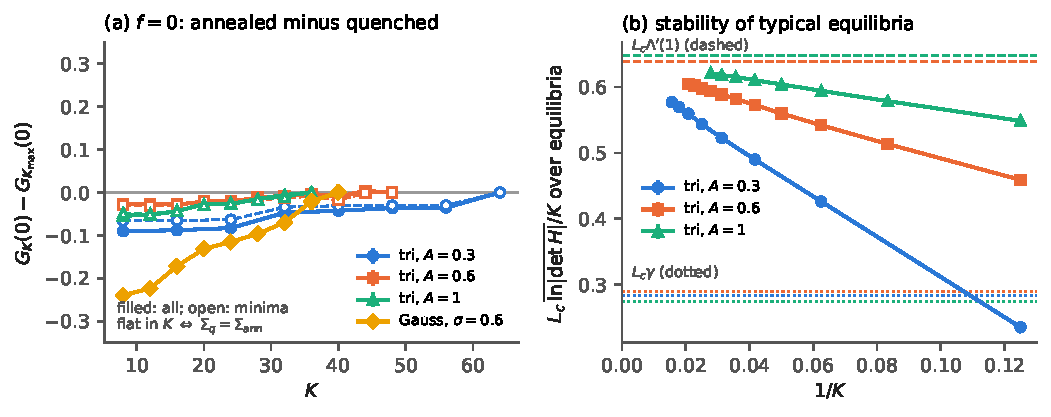
\includegraphics[width=\textwidth]{fig1_zero_force.pdf}
\caption{(a) $G_K$ at $f=0$, offset by its value at $K_{\max}$, for all equilibria (filled) and minima (open, triangle model). A flat $G_K$ means $\Sq=\Sann$; the growth for Gaussian disorder is the amplitude effect. (b) The mean of $\ln|\det H|/K$ over the equilibria of a sample tends to $\Lambda'(1)$ (dashed), not to the Lyapunov exponent $\gamma$ (dotted).}
\label{fig:zero}
\end{figure}

\paragraph{Finite force.}
In the tilt-symmetry frame, the small-$f$ behaviour is set by the level profile of a typical sample.
Let $c_s$ be its centre and $K\chi_q$ its variance, and define $\chi_c=\langle c_s^2\rangle/K$.
The exact Kac--Rice result gives $\chi_q+\chi_c\to\langle V'^2\rangle$.
A quadratic gap $\Sann-\Sq\simeq f^2\chi_c/(2\chi(\chi-\chi_c))$ would therefore require an extensive common offset.
It is absent: $\langle c_s^2\rangle$ grows only from $0.11$ to $0.18$ for $K=8\to32$, so $\chi_c\to0$ and $\Sq=\Sann+o(f^2)$ (Fig.~\ref{fig:loc}b).

At larger $f$, $\Sq$ and $\Sann$ agree within $1$--$3\%$ up to $f\approx0.6$--$0.7\,f_c$ (Fig.~\ref{fig:force}).
The larger residual, at $A=0.3$, comes with the slow logarithmic drift of $G_K(0)$ at that disorder strength.
The gap is $\approx6\%$ of $\Sann$ at $0.8\,f_c$ and about $20\%$ at $0.9\,f_c$ in all three triangle models. Above $f_c$ there are no equilibria, while $\Sann(f_c)\approx0.6\,\Sann(0)$. Just below $f_c$, $\Sq$ does not go to zero (Sec.~\ref{sec:jump}).

For Gaussian disorder, the reference curve is the amplitude-quenched $\Sigma_{\rm sa}$ rather than $\Sann$.
$\Sq$ follows $\Sigma_{\rm sa}$ to within $0.2$--$1.7\%$, about $1\sigma$, up to $0.6\,f_c$.
It then departs in the same way as the triangle model departs from $\Sann$: by $4\%$ at $0.7\,f_c$, $8.5\%$ at $0.8\,f_c$ and $21\%$ at $0.9\,f_c$.
Two mechanisms are therefore at work and can be separated:
\begin{itemize}
\item the shared site amplitudes give a small Jensen gap at all forces, which is computed exactly;
\item the localization of the leading edge in $u$ gives the large gap near threshold.
\end{itemize}
Minima behave in the same way.
At the present sizes we cannot tell whether the onset is a sharp transition at some $f_*<f_c$ or a fast crossover.

\begin{figure}[H]
\centering
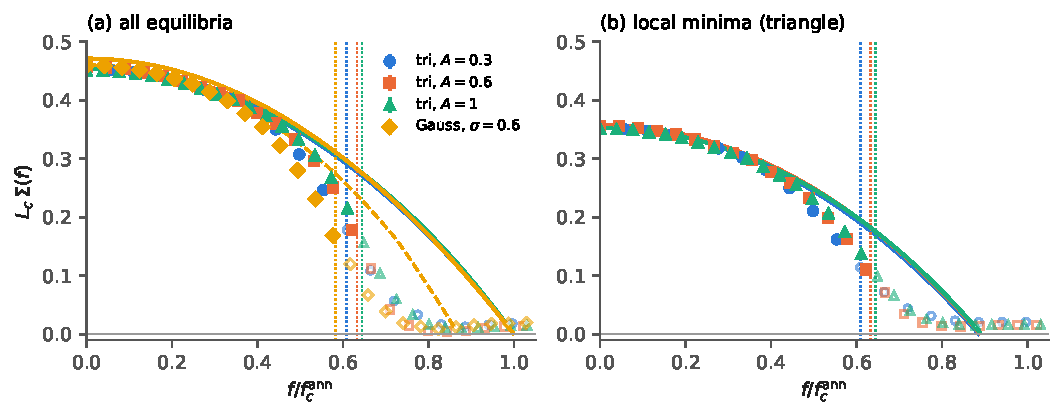
\includegraphics[width=\textwidth]{fig2_force.pdf}
\caption{Complexity versus force. Lines: exact annealed rates. Markers: quenched rates $\Sann-b$; error bars are fit errors only. Dotted verticals: thresholds $f_c$ ($\nu=4/3$ fit). Open markers above $f_c$ are finite-$K$ residue; just below $f_c$, the finite-force estimator is rounded by sample-to-sample threshold fluctuations (see Sec.~\ref{sec:jump}).}
\label{fig:force}
\end{figure}

\begin{table}[H]
\centering\footnotesize\setlength{\tabcolsep}{3.5pt}
\begin{tabular}{lcccccccc}
\toprule
model & $f_c^{\rm ann}$ & $f_c^{\rm ann,min}$ & $f_c$ ($\nu=4/3$) & $f_c$ (front) & $f_c$ (free $\nu$) & $\nu$ & $\omega$ & $f_c^{\rm ann}/f_c$ \\
\midrule
\csname @@input\endcsname table_threshold.tex
\bottomrule
\end{tabular}
\caption{Thresholds. $f_c^{\rm ann}$ and $f_c^{\rm ann,min}$ are the zeros of $\Sann$ and $\Sann^{\rm min}$. $f_c$ is extrapolated from $\langle\max_aW_K\rangle/K$ for $K\ge12$ in three ways: $f_c+cK^{-1/\nu}$ with $\nu=4/3$; the branching-front form $f_c+a\ln K/K+b/K$; and free $\nu$. $\omega$ is the exponent of the sample-to-sample spread, ${\rm sd}\,f_c(K)\propto K^{-\omega}$. The last column spans the three fits.}
\label{tab:thr}
\end{table}

\paragraph{Threshold.}
$f_c^{\rm ann}/f_c$ is $1.57$--$1.64$ at the weakest disorder, against FLRT's dynamical $1.64\pm0.02$ (Fig.~\ref{fig:thr}b, Table~\ref{tab:thr}).
It is $1.5$--$1.58$ at $L_c\le1.4$, where lattice corrections are larger.
Exact thresholds of chains up to $K=1024$ (Sec.~\ref{sec:relax}) settle the extrapolation: $1.59$, $1.55$ and $1.51$ at $L_c=2.2$, $1.4$ and $1$, i.e.\ the front and free-$\nu$ fits, not the $\nu=4/3$ one.
For Gaussian disorder at $L_c=1.41$ it is $1.65$--$1.72$: the amplitude fluctuations lower $f_c$ further.
The spread comes from the extrapolation form: the $\nu=4/3$ fit gives the lowest $f_c$, while the branching-front and free-$\nu$ fits agree with each other.
Counting minima tightens the bound to $f_c^{\rm ann,min}$, but it remains far from tight.

The sample threshold fluctuates as $K^{-\omega}$ with $\omega=0.50\pm0.02$ in all models.
That is the scaling of the maximum of a branching structure in a \emph{time-random} environment (Mallein--Miłoś), not $K^{-1/\nu}$.
As in FLRT's torus geometry, the period of the medium is fixed while $K$ grows, so this $f_c$ is the threshold of a $u$-periodic medium.

\begin{figure}[H]
\centering
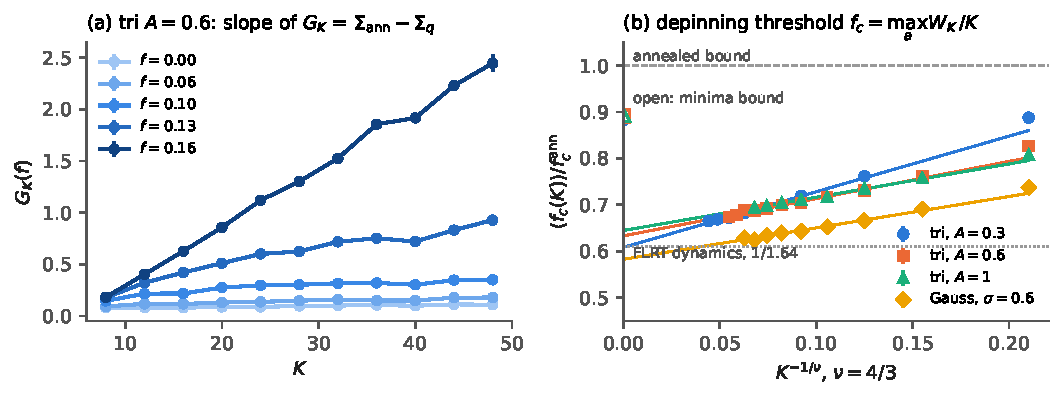
\includegraphics[width=\textwidth]{fig3_threshold.pdf}
\caption{(a) $G_K(f)$ for the triangle model at $A=0.6$. The slope is $\Sann-\Sq$; it is zero up to $f\approx0.1$ and positive beyond. (b) Mean sample threshold $\langle\max_aW_K\rangle/K$ in units of $f_c^{\rm ann}$, with $\nu=4/3$ fits. Open: minima bound. Dotted: FLRT's $1/1.64$.}
\label{fig:thr}
\end{figure}

\section{Theory}\label{sec:theory}

By Eq.~\eqref{eq:sts} the problem is a branching structure at zero force: the folds of the shooting curve, located at positions $W$ (the accumulated force).
The branching takes place in an environment, the functions $V_i$, that is random in ``time'' $i$ but shared by all branches at a given generation.
Branches see different forces only through their positions $u$ mod $P$.
This section turns that picture into exact statements, bounds and a mechanism, each checked against the counts.

\subsection{Partition function and quenched pressure}

Since $|\det H(a)|=|W_K'(a)|$, the coarea formula gives
\begin{equation}
Z_K(\tau)\equiv\int_0^P\!da\;e^{\tau W_K(a)}\,|\det H(a)|=\int\!dx\;N_K(x)\,e^{\tau x},
\label{eq:Z}
\end{equation}
so the level counts determine $Z$ and conversely.
Its average is exact: in the triangle model $\langle Z_K(\tau)\rangle=P\,\langle e^{\tau V'}\rangle^K\langle|D_K|\rangle$, so
\[
\Lambda(\tau)\equiv\lim K^{-1}\ln\langle Z_K\rangle=\Lambda(1)+\ln\frac{\sinh\tau A}{\tau A}.
\]
For the Gaussian model, $\Lambda(\tau)$ is the top eigenvalue of the tilted operator.

The quenched pressure $\varphi_q(\tau)=\lim K^{-1}\langle\ln Z_K(\tau)\rangle$ is convex, with $\varphi_q\le\Lambda$.
When $\Sq$ is concave, the two are related by a Legendre transform:
\begin{equation}
\Sq(v)=\inf_\tau\big[\varphi_q(\tau)-\tau v\big],\qquad
\varphi_q(\tau)=\sup_{v\le f_c}\big[\Sq(v)+\tau v\big].
\label{eq:legendre}
\end{equation}
Two consequences:
\begin{itemize}
\item $\varphi_q(0)=\Sq(0)$;
\item at large $\tau$, $\varphi_q(\tau)=\Sq(f_c^-)+\tau f_c+o(1)$, so the threshold is the asymptotic slope of the quenched pressure.
\end{itemize}
Equivalently, $f_c$ is the largest ergodic average of the force $V_i'(u_i)$ over orbits of the random twist map.

We estimate $\varphi_q$ from the level counts, Eq.~\eqref{eq:Z}, using the slope of $\ln\langle Z_K\rangle-\langle\ln Z_K\rangle$ in $K$.
At large $\tau$ it is linear (Table~\ref{tab:theory}):
\begin{itemize}
\item its slope reproduces the extrapolated $f_c$ in all four models;
\item its intercept is positive, which is the content of Sec.~\ref{sec:jump}.
\end{itemize}

\subsection{Exact bounds}

For any sub-$\sigma$-algebra $\mathcal G$ of the disorder, Jensen's inequality for conditional expectations gives $\langle\ln N\rangle\le\langle\ln\langle N|\mathcal G\rangle\rangle$.
Take for $\mathcal G$ the site amplitudes $R_i$.
At fixed amplitudes the phases are still independent, so Kac--Rice factorises as before:
\[
\langle N_K|R\rangle=P\,p_{S_K|R}(Kf)\,\|T_{R_K}\cdots T_{R_1}\|,
\]
where $T_R$ is the phase-averaged transfer operator at amplitude $R$.
Hence, rigorously,
\begin{equation}
\Sq(f)\le\Sigma_{\rm sa}(f)\le\Sann(f),\qquad f_c\le f_{\rm sa}\le f_c^{\rm ann},
\label{eq:bounds}
\end{equation}
with $\Sigma_{\rm sa}(f)=\inf_\tau[\Lambda_q(\tau)-\tau f]$ and $\Lambda_q(\tau)$ the Lyapunov exponent of the tilted random operator product.

For the triangle model $T_R$ is non-random, so $\Sigma_{\rm sa}=\Sann$.
For the Gaussian model, $f_{\rm sa}=0.423\pm0.001$ against $f_c^{\rm ann}=0.486$, and at $f=0$ the bound is saturated within errors (Sec.~6, zero force with random amplitude).

This splits FLRT's ratio into two factors:
\begin{itemize}
\item the shared amplitudes account for $f_c^{\rm ann}/f_{\rm sa}=1.15$;
\item the rest, $f_{\rm sa}/f_c=1.43$--$1.49$, is of the same size as the whole ratio in the triangle model at the same $L_c$ ($1.55$--$1.58$), where amplitudes play no role.
\end{itemize}

\subsection{Population dynamics and the Jensen gap}

Write $Z_K=Z_0\prod_im_i$ with $m_i=Z_{i+1}/Z_i$.
The tilted population at site $i$ is a measure $\rho_i$ on $(u\bmod P,\,w\bmod P,\,\theta)$, where $\theta$ is the tangent angle.
Its dynamics closes on this compact space, because $u_{i+1}=u_i+w_i$ only needs $w\bmod P$.
For a fixed amplitude, averaging over the fresh phase at site $i$ at fixed past gives
\begin{equation}
\langle m_i\,|\,{\rm past}\rangle=\int d\theta\,\rho_i(\theta)\,\kappa_\tau(\theta),\qquad
\kappa_\tau(\theta)=\langle e^{\tau V'}\,|M_Uv_\theta|\rangle ,
\end{equation}
which depends only on the angle marginal of $\rho_i$.
The annealed pressure is obtained exactly when $\rho_i$ is uniform in $u$ and its angle marginal is the stationary one of the annealed operator: then $m_i$ is non-random and equals $e^{\Lambda(\tau)}$.
The quenched pressure is $\lim K^{-1}\sum_i\langle\ln m_i\rangle$, and the Jensen gap per site is, to second order,
\begin{equation}
\Lambda(\tau)-\varphi_q(\tau)\simeq\frac12\sum_{n\ne0}\big\langle|\hat\rho_{i,n}|^2\big\rangle\,\frac{|\hat\kappa_n|^2}{\hat\kappa_0^2},
\label{eq:jgap}
\end{equation}
where $\hat\rho_{i,n}$ are the $u$-Fourier components of the population and $\hat\kappa_n$ those of $e^{\tau V'(u)}|M_{U(u)}v|$ over one period.

In the continuum limit both factors vanish at $\tau=0$:
\begin{itemize}
\item the non-uniformity $\hat\rho_n$ is created by the tilt and erased by the shear $u\to u+w$, so $\langle|\hat\rho_n|^2\rangle=O(\tau^2)$;
\item $\hat\kappa_n=O(\tau)$.
\end{itemize}
The gap is therefore $O(\tau^4)$, so $\Sann-\Sq=o(f^2)$, which is what the non-extensive sample centre showed.
The measured gap grows as $\tau^{3}$--$\tau^{4}$ (Fig.~\ref{fig:theory}a), not as $\tau^2$.

On the lattice, the stretching factor $|M_{U(u)}v|$ depends on the cell even at $\tau=0$, so $\hat\kappa_n$ and $\hat\rho_n$ are small but nonzero there.
This leaves a small zero-force gap: $0.0004$ at $A=0.6$ and $0.0019$ at $A=1$ (torus, below), i.e.\ $0.1$--$0.4\%$ of $\Sigma(0)$.
It matches the enumeration ($0.0012\pm0.0008$ and $0.0021\pm0.0009$), shrinks quickly with $A$, and vanishes in the continuum limit.
"Quenched = annealed at $f=0$" for fixed amplitude is therefore exact only in that limit; on the lattice it holds to $\lesssim0.5\%$.

As $\tau$ grows, the tilted population concentrates on fewer lineages, $\rho_i$ stops being uniform in $u$, and the gap becomes of order one.
This is the weak-to-strong-disorder transition of a branching process in a time-random environment, or of a directed polymer.
The equilibria localise in $u$ (Fig.~\ref{fig:loc}a), and the onset sits at $f\approx0.75f_c$.

If lineages decorrelated as soon as they split, as in a branching random walk, the onset would be at the annealed edge $f_c^{\rm ann}$.
Even the second-moment bound would hold up to $I(f)=\Lambda(1)/2$, i.e.\ $0.71f_c^{\rm ann}$.
The earlier onset comes from the shared environment: lineages at the same $u$ mod $P$ see the same force without being related.

\begin{figure}[H]
\centering
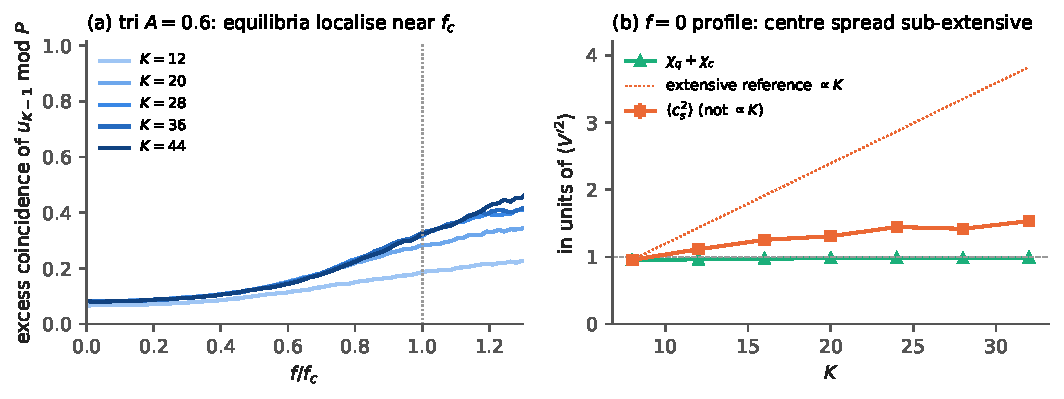
\includegraphics[width=\textwidth]{fig4_localisation.pdf}
\caption{(a) Excess pair coincidence of the end positions $u_{K-1}$ mod $P$ of the equilibria of a sample, over independent uniform positions; 0 means spread, 1 means a single cluster. The $f=0$ baseline ($\approx0.08$, independent of $K$) is the free-end boundary layer. (b) Level profile at $f=0$, triangle $A=0.6$: the mean-square sample centre $\langle c_s^2\rangle$ is not extensive, and $\chi_q+\chi_c\to\langle V'^2\rangle$.}
\label{fig:loc}
\end{figure}

\subsection{Replicated Kac--Rice}\label{sec:replica}

The quenched rate is the $n\to0$ limit of the moments $\langle Z_K(\tau)^n\rangle$, and for integer $n$ these are Kac--Rice integrals over $n$ replicas in the same environment.
In the triangle model they reduce exactly to transfer operators, which we now set up.

\paragraph{Replica operator.}
By Eq.~\eqref{eq:Z},
\begin{equation}
\langle Z_K(\tau)^n\rangle=\int_{[0,P)^n}\prod_{\alpha=1}^n da_\alpha\;\Big\langle\prod_\alpha e^{\tau W_K(a_\alpha)}\,|\psi_K(a_\alpha)|\Big\rangle ,
\label{eq:Zn}
\end{equation}
with $\psi$ the Gelfand--Yaglom tangent, $\psi_{i+1}=(2+V_i''(u_i))\psi_i-\psi_{i-1}$.
At site $i$ write $u^\alpha_i-\phi_i=\theta_i+s^\alpha_i$, where $\theta_i$ is the position of replica 1 relative to the fresh phase, uniform and independent of the past, and $s^\alpha_i=u^\alpha_i-u^1_i$ mod $P$ are the offsets.
The replicas see the forces $g(\theta_i+s^\alpha_i)$ and the slopes $\pm k$ of a single triangle wave $g$, and the offsets move as
\begin{equation}
d^\alpha_{i+1}=d^\alpha_i+g(\theta_i+s^\alpha_i)-g(\theta_i),\qquad s^\alpha_{i+1}=s^\alpha_i+d^\alpha_{i+1}\pmod P .
\end{equation}
So Eq.~\eqref{eq:Zn} is a Feynman--Kac average over a Markov chain on $(s^\alpha,d^\alpha)_{\alpha\ge2}\in\mathbb T^{2(n-1)}$ and $n$ projective tangents, with site weight $\prod_\alpha e^{\tau g(\theta_i+s^\alpha_i)}\|\psi^\alpha_{i+1}\|/\|\psi^\alpha_i\|$.
Hence $\langle Z_K^n\rangle\asymp e^{K\Lambda_n(\tau)}$, with $\Lambda_n$ the log top eigenvalue of an explicit $n$-replica operator, and $\varphi_q=\lim_{n\to0}\Lambda_n/n$.
Since $(\langle Z^n\rangle)^{1/n}$ increases with $n$, $\varphi_q\le\Lambda_n/n$ for every $n>0$. Integer $n\ge1$ only reproduce the annealed bound $\Lambda_1=\Lambda$.

\paragraph{Exact structure.}
\begin{itemize}
\item \textbf{$n=1$} has no offsets. Force and slope at a uniform point are independent, so $\Lambda_1(\tau)=\Lambda(1)+\ln[\sinh(\tau A)/\tau A]$, the FLRT result.
\item \textbf{The offset chain preserves area.} Each step is a composition of two shears of the torus, so the unweighted chain leaves the uniform measure invariant. For uniformly spread offsets the pair force weight factorises exactly:
\[\int_0^P\frac{ds}{P}\,\big\langle e^{\tau[g(\theta)+g(\theta+s)]}\big\rangle_\theta=\langle e^{\tau g}\rangle^2 .\]
 Any excess $\Lambda_2-2\Lambda$ therefore comes from correlations: from the non-uniform law of the offsets of pairs that meet again on the torus, and from the shared slope signs of nearby replicas.
\item \textbf{Locked pairs.} Replicas with $|a-a'|\lesssim1/|\psi_K(a)|$ follow the same trajectory. They contribute
\[\int da\;e^{2\tau W}\,\frac{|\psi_K|^2}{|\psi_K|}=Z_K(2\tau),\qquad\text{so}\quad \Lambda_2(\tau)\ge\max[2\Lambda(\tau),\Lambda(2\tau)].\]
\end{itemize}

\paragraph{The second-moment window, in closed form.}
Where $\Lambda_2=2\Lambda$, Paley--Zygmund gives $P(Z_K\ge\langle Z_K\rangle/2)\ge e^{-o(K)}$, and with the almost-sure convergence of $K^{-1}\ln Z_K$ (Furstenberg--Kesten) this forces $\varphi_q=\Lambda$.
The locked pairs alone close this window at $2\Lambda(\tau)=\Lambda(2\tau)$, i.e.
\begin{equation}
x\coth x=e^{\Lambda(1)},\qquad x=\tau A .
\label{eq:L2}
\end{equation}
This gives $x_\times=0.84$, $1.12$ and $1.39$ for $A=0.3$, $0.6$ and $1$; the annealed force there is $0.74$--$0.79\,f_c^{\rm ann}$.
In the continuum limit, $\Lambda(1)=C/L_c\to0$, Eq.~\eqref{eq:L2} gives $x_\times^2=3\Lambda(1)$ against $x_c^2=6\Lambda(1)$ at the annealed threshold, so the window ends at $f_\times\to f_c^{\rm ann}/\sqrt2$. This is the $L^2$ boundary of the directed polymer on a tree (Derrida--Spohn), here exact.

\paragraph{The pair operator.}
We computed $\Lambda_2(\tau)$ by population dynamics of the pair operator ($2\times10^5$ walkers, $3000$ sites; \texttt{replica.py}). The same code reproduces $\Lambda_1$ to $10^{-4}$. Two regimes appear (Fig.~\ref{fig:replica}a):
\begin{itemize}
\item \textbf{Replica symmetric}, up to $\tau A\approx0.5$, $0.75$ and $1$ for $A=0.3$, $0.6$ and $1$: the excess $\varepsilon(\tau)=\Lambda_2-2\Lambda$ is small, $0.001$--$0.02$, and grows smoothly from a non-zero value at $\tau=0$.
\item \textbf{Correlated pairs}, beyond these values but still \emph{before} $x_\times$: $\Lambda_2$ rises steeply and soon exceeds even the locked value. At $A=0.3$, $\Lambda_2-\Lambda(2\tau)=0.050\pm0.002$ for all $\tau A\ge1.25$; at $A=0.6$ and $1$ the difference is still decreasing toward a plateau at $\tau A=2$. The pair moment is then carried by pairs that travel together, separate and lock again. Population dynamics cannot sample pairs locked over the whole chain (their initial offsets are $e^{-\lambda K}$), so here the computed $\Lambda_2$ is a lower bound.
\end{itemize}

\paragraph{Replica Gaussian closure.}
If $\ln Z_K$ is Gaussian with variance $K\sigma^2$, then $\Lambda_n=n\varphi_q+n^2\sigma^2/2$, so
\begin{equation}
\Lambda-\varphi_q=\frac{\sigma^2}2=\frac{\Lambda_2-2\Lambda}2 .
\label{eq:closure}
\end{equation}
All three quantities are measured independently: the gap from $\langle\ln Z\rangle$, $\sigma^2$ from ${\rm Var}\ln Z_K$ in the enumeration, and $\varepsilon$ from the pair operator.
They agree in the replica-symmetric regime (Fig.~\ref{fig:replica}b). At $A=1$:
\begin{center}\footnotesize
\begin{tabular}{lccccc}
\toprule
$\tau A$ & 0 & 0.25 & 0.5 & 0.75 & 1 \\
\midrule
$\varepsilon/2$ (pair operator) & 0.0023 & 0.0026 & 0.0041 & 0.0085 & 0.0196 \\
$\sigma^2/2$ (enumeration) & 0.0023 & 0.0027 & 0.0043 & 0.0083 & 0.0162 \\
gap (enumeration) & 0.0021(9) & 0.0025(10) & 0.0042(12) & 0.0084(16) & 0.0169(22) \\
\bottomrule
\end{tabular}
\end{center}
The closure also accounts for the lattice gap at zero force (Sec.~7.3): there $\varepsilon/2=0.0005$ and $0.0023$ at $A=0.6$ and $1$, against the measured $0.0012\pm0.0008$ and $0.0021\pm0.0009$. Its origin is now explicit: nearby replicas share slope signs, so their stretch factors are correlated.
The gap keeps following $\sigma^2/2$ up to $\tau A\approx1$, while $\varepsilon/2$ overshoots once correlated pairs dominate. Beyond $\tau A\approx1.2$ the gap exceeds $\sigma^2/2$ as well, because the left tail of $\ln Z$ is no longer Gaussian.

\paragraph{The threshold needs replica symmetry breaking.}
\begin{itemize}
\item The closure, Eq.~\eqref{eq:closure}, applied at all $\tau$ with the measured $\sigma^2(\tau)$, predicts $f_c\simeq\min_\tau[\Lambda(\tau)-\sigma^2(\tau)/2]/\tau=0.095$, $0.248$ and $0.439$ for $A=0.3$, $0.6$ and $1$, against the exact $0.068$, $0.175$ and $0.346$ (Sec.~\ref{sec:relax}). It accounts for only a third of the drop from $f_c^{\rm ann}$.
\item A one-step RSB ansatz in which the $n$ replicas form $n/m$ independent clusters of $m$ locked replicas gives $\langle Z^n\rangle\asymp e^{K(n/m)\Lambda(m\tau)}$, hence $\varphi_q=\min_{0<m\le1}\Lambda(m\tau)/m$. This is Derrida--Spohn freezing: $f_c=f_c^{\rm ann}$ and $c=0$. It is the exact answer on a tree, where clusters never meet again.
\end{itemize}
So the whole ratio $f_c^{\rm ann}/f_c\approx1.6$ comes from correlations \emph{between} clusters, i.e.\ from distinct near-critical strands meeting again in the shared, bounded environment on the torus. This is the replica form of the localisation mechanism of Sec.~7.3. It is also consistent with the positive jump $c$ (Sec.~\ref{sec:jump}): the frozen phase is a non-trivial cluster of strands, not a single one.
A quantitative theory of $f_c$ needs this inter-cluster interaction at $m<1$. The next subsection turns it into rigorous bounds.

\begin{figure}[H]
\centering
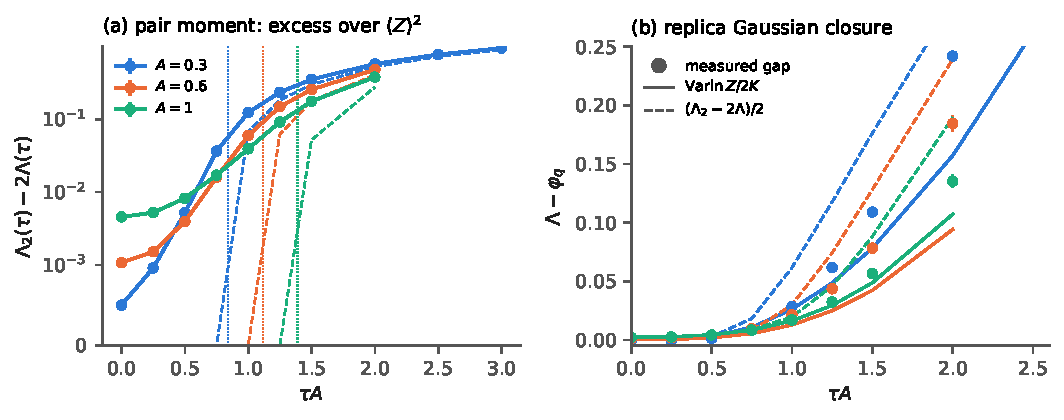
\includegraphics[width=\textwidth]{fig10_replica.pdf}
\caption{Replicated Kac--Rice, triangle model. (a) Excess of the pair moment over $\langle Z\rangle^2$ (markers), the locked-pair value $\Lambda(2\tau)-2\Lambda(\tau)$ (dashed) and the second-moment boundary $x_\times$ of Eq.~\eqref{eq:L2} (dotted). (b) Measured quenched--annealed gap (markers), ${\rm Var}\ln Z_K/2K$ (solid) and $(\Lambda_2-2\Lambda)/2$ (dashed): the Gaussian closure, Eq.~\eqref{eq:closure}.}
\label{fig:replica}
\end{figure}

\subsection{Fractional moments and change of measure: rigorous bounds below the annealed threshold}\label{sec:fracbound}

\paragraph{The bound.}
For any positive function $G$ of the disorder and $0<m<1$, Jensen and Hölder give
\[
\langle\ln Z\rangle\le\frac1m\ln\langle Z^m\rangle\le\frac{1-m}{m}\ln\big\langle G^{-m/(1-m)}\big\rangle+\ln\langle GZ\rangle .
\]
Take $G=dQ/dP$ for a second disorder law $Q$. The first term increases with $m$, so the best choice is $m\to0$, where it becomes the relative entropy:
\begin{equation}
\varphi_q(\tau)\le B_Q(\tau)\equiv\Lambda_Q(\tau)+d(P\|Q),\qquad f_c\le\inf_\tau\frac{B_Q(\tau)}{\tau}.
\label{eq:cmbound}
\end{equation}
Here $\Lambda_Q$ is the annealed rate under $Q$ and $d$ the relative entropy per site. $Q=P$ gives back the annealed bounds.
The family is complete: block tilts $G=\mathbf 1_E+\delta$, with $E$ the event that $\ln Z$ is typical on a block, make Eq.~\eqref{eq:cmbound} tight as the block length grows. What matters in practice is how fast it converges.

\paragraph{A computable family.}
Phases $\phi_i$ iid uniform are equivalent to second differences $V_i=\phi_i-2\phi_{i-1}+\phi_{i-2}$ iid uniform on $[0,P)$.
A strand's position relative to the phase, $\theta_i=u_i-\phi_i$, obeys the shooting map
\begin{equation}
\theta_{i+1}=2\theta_i-\theta_{i-1}+g(\theta_i)-V_{i+1}\pmod P ,
\end{equation}
so tilting the law of the $V_i$ changes which orbits are available.
\begin{itemize}
\item \textbf{iid tilt}, $V_i\sim h(v)/P$: $d=-\langle\ln h\rangle$, and $\Lambda_Q$ is the top eigenvalue of an operator on $(\theta_i,\theta_{i-1})$ and the tangent direction (\texttt{fracbound.py}; $96^2\times48$ grid, exact $\Lambda$ reproduced to $2\times10^{-4}$ at $h=1$).
\item \textbf{Markov tilt}, $V_{i+1}|V_i\sim h(V_i,V_{i+1})/P$: $V_i$ is fixed by $(\theta_i,\theta_{i-1},\theta_{i-2})$, so the operator acts on three positions and the tangent (\texttt{fracbound2.py}; $48^3\times24$ grid).
\end{itemize}
We optimise $\ln h$ over Fourier modes up to order 4 (iid) and 2 in each argument (Markov), jointly with $\tau$ for the threshold. The grid error of the flat operator is subtracted.

\begin{table}[H]
\centering\footnotesize
\begin{tabular}{lccc}
\toprule
$A$ & 0.3 & 0.6 & 1 \\
\midrule
$f_c^{\rm ann}$ & 0.1084 & 0.2704 & 0.5240 \\
bound, iid tilt & 0.1080 & 0.2660 & 0.4990 \\
bound, Markov tilt & 0.1074 & 0.2621 & 0.4887 \\
exact $f_c$ (Sec.~\ref{sec:relax}) & 0.0682 & 0.1749 & 0.3460 \\
fraction of $f_c^{\rm ann}-f_c$ closed (iid, Markov) & 1\%, 2.5\% & 5\%, 9\% & 14\%, 20\% \\
\midrule
$\Lambda-B$ at $\tau A=1,\,2,\,3$ (iid) & 0.001, 0.017, 0.074 & 0.002, 0.026, 0.095 & 0.008, 0.047, 0.138 \\
measured $\Lambda-\varphi_q$ at $\tau A=1,\,2,\,3$ & 0.028, 0.242, 0.625 & 0.021, 0.184, 0.515 & 0.017, 0.135, 0.402 \\
\bottomrule
\end{tabular}
\caption{Change-of-measure bounds, Eq.~\eqref{eq:cmbound}, for the triangle model.}
\label{tab:cmbound}
\end{table}

\paragraph{Results.}
\begin{itemize}
\item \textbf{The annealed threshold is not sharp.} Every tilt gives $f_c<f_c^{\rm ann}$ rigorously, up to the grid discretisation. With one step of memory the ratio is bounded below by $f_c^{\rm ann}/f_c\ge1.009$, $1.032$ and $1.072$ at $A=0.3$, $0.6$ and $1$. The bound needs no simulation of the quenched problem: only the top eigenvalue of an annealed operator.
\item \textbf{The gain grows with pinning strength}, from $1\%$ to $20\%$ of the true gap at $A=0.3\to1$. The pressure bound closes $4\%$, $10\%$ and $47\%$ of the measured gap at $\tau A=1$ (for $A=0.3$, $0.6$, $1$), and $12$--$34\%$ at $\tau A=3$.
\item \textbf{The gain grows with memory.} Adding one step of memory to the tilt doubles the part of the gap closed at weak pinning. The orbits that set $f_c$ are correlated over $L_c$ sites ($2.2$, $1.4$ and $1$ here), and a tilt only sees as many consecutive phases as its memory. Single-site tilts therefore fail at weak pinning, the regime FLRT consider. This is the same statement as the replica one: the gap lives in correlations between strands over many sites, not in the single-site law.
\end{itemize}
So the rigorous route works, and it is quantitative at moderate pinning. At weak pinning, Eq.~\eqref{eq:cmbound} needs tilts with memory of many $L_c$, which the next paragraph constructs.

\paragraph{Block tilts.}
Cut the second differences into blocks of $\ell$ consecutive $V_i$. For any positive block function $Z_b(V_{\rm block})$ take $G=\prod_bZ_b^{-\lambda}/\langle Z_b^{-\lambda}\rangle$. The normalisations cancel against the relative entropy, and Eq.~\eqref{eq:cmbound} becomes
\begin{equation}
\varphi_q(\tau)\le B_\ell(\tau)=\lim_{K\to\infty}\frac1K\ln\Big\langle Z_K\prod_bZ_b^{-\lambda}\Big\rangle+\frac{\lambda}{\ell}\langle\ln Z_b\rangle ,
\label{eq:blockbound}
\end{equation}
for every $\ell$, $\lambda$ and every choice of $Z_b$. The tilt penalises blocks in which many orbits do well. We take for $Z_b$ the quenched partition function of the block alone,
\[
Z_b=\frac1{P^2}\int_0^P\!\!d\theta_0\int_0^P\!\!d\theta_{-1}\;e^{\tau\sum_{j=1}^{\ell}g(\theta_j)}\,\|M_\ell\|_F ,
\]
with the orbit started from every entry state and $M_\ell$ the tangent product over the block. Three ingredients make Eq.~\eqref{eq:blockbound} computable:
\begin{itemize}
\item \textbf{Exact $Z_b$.} The block map is affine on convex polygons of entry states, so $Z_b$ is a finite sum of exponential integrals over polygons, traced exactly (\texttt{blockbound.py}). Polygons below $e^{-30}$ of the running total are dropped; the rule is deterministic, so $Z_b$ stays a fixed function of $V$. It agrees with a $600^2$ grid to grid accuracy.
\item \textbf{Planted strands.} By stationarity $\langle Z_KF(V)\rangle=P\langle e^{\tau W_K(0)}|\psi_K(0)|F(V)\rangle$, and along the strand $a=0$ the $\theta_i$ are iid uniform, with the $V_i$ functions of them. The first term is therefore the growth rate of a population of planted strands: $\theta_i$ drawn from the law $\propto e^{\tau g}$, weighted by the tangent growth and, at each block end, by $Z_b^{-\lambda}$ of the block they have generated. At $\lambda=0$ it reproduces $\Lambda(\tau)$ to $5\times10^{-4}$.
\item \textbf{Why it can be tight.} With $\lambda=1$, a planted strand contributes its own weight to its block's $Z_b$. The first term is then expected to stay $O(1/\ell)$, so that $B_\ell$ approaches the block-quenched pressure $\langle\ln Z_b\rangle/\ell\to\varphi_q$ (a heuristic, not a proof: the strand's share of $Z_b$ can be small). We use $\lambda=1$; in tests at $A=0.3$, $\ell=16$, $\lambda=0.7$ and $1.3$, and $Z_b$ evaluated at $0.7\tau$ or $1.4\tau$, all give weaker bounds.
\end{itemize}

\begin{table}[H]
\centering\footnotesize
\begin{tabular}{lcccccc}
\toprule
& \multicolumn{2}{c}{$A=0.3$} & \multicolumn{2}{c}{$A=0.6$} & \multicolumn{2}{c}{$A=1$} \\
$\ell$ & $\tau A=2$ & $3$ & $2$ & $3$ & $2$ & $3$ \\
\midrule
1 (single-site tilt) & 0.07 & 0.12 & 0.14 & 0.18 & 0.35 & 0.34 \\
4 & 0.08 & 0.13 & 0.14 & 0.19 & 0.27 & 0.28 \\
8 & 0.24 & 0.32 & 0.35 & 0.40 & 0.54 & 0.53 \\
16 & 0.43 & 0.55 & 0.54 & 0.66 & 0.76 & 0.82 \\
\midrule
measured $\Lambda-\varphi_q$ & 0.242 & 0.625 & 0.184 & 0.515 & 0.135 & 0.402 \\
\bottomrule
\end{tabular}
\caption{Fraction $(\Lambda-B_\ell)/(\Lambda-\varphi_q)$ of the measured pressure gap closed by block tilts, Eq.~\eqref{eq:blockbound}. Row $\ell=1$ is the optimised single-site tilt of Table~\ref{tab:cmbound}. Each entry is stable between populations of $2000$ and $8000$ planted strands.}
\label{tab:block}
\end{table}

\begin{figure}[H]
\centering
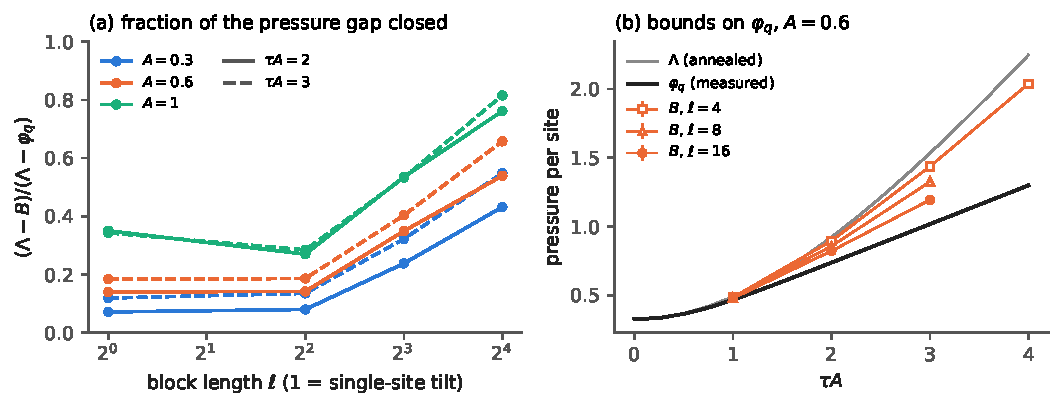
\includegraphics[width=\textwidth]{fig11_block.pdf}
\caption{Block change-of-measure bounds. (a) Fraction of the pressure gap closed against block length, at $\tau A=2$ (solid) and $3$ (dashed). (b) Bounds $B_\ell(\tau)$ at $A=0.6$ between the annealed and the measured quenched pressure; only points stable in the population size are shown.}
\label{fig:block}
\end{figure}

\paragraph{Results of the block tilts.}
\begin{itemize}
\item \textbf{The pressure gap is captured.} At $\ell=16$ the bound closes about half of the measured gap at weak pinning and two thirds or more at stronger pinning (Table~\ref{tab:block}), against $7$--$35\%$ for the best single-site tilt. The fraction grows by about $0.2$ per doubling of $\ell$. In units of the Larkin length, $\ell=16$ is $7$, $11$ and $16\,L_c$. So the quenched--annealed gap is carried by phase correlations over about ten Larkin lengths, not by the single-site law.
\item \textbf{Threshold.} The best stable bounds are $f_c\le0.1043$, $0.2386$ and $0.4437$ at $A=0.3$, $0.6$ and $1$, closing $10$, $33$ and $45\%$ of the gap from $f_c^{\rm ann}$ to the exact $f_c$ (Markov tilt: $2.5$, $9$ and $20\%$). For the threshold alone this is not the best tool. As $\tau\to\infty$ the bound reduces to the subadditive block bound $f_c\le\langle\max_{\rm orbits}\sum_jg(\theta_j)\rangle/\ell$, so it cannot beat finite-block maxima, and the relaxation thresholds of Sec.~\ref{sec:relax} remain the accurate route to $f_c$. What the block tilt adds is the pressure at finite $\tau$, and with it an upper bound on $\Sq(f)$ that lies well below the annealed curve.
\item \textbf{The limit is statistical, not analytic.} Eq.~\eqref{eq:blockbound} is a theorem for every $\ell$; the bottleneck is its evaluation. A strand's block weight divided by $Z_b$ is the posterior density of its entry state given the block. Its mean is exact, but its distribution has a tail up to $e^{\gamma\ell}$, with $\gamma$ the Lyapunov exponent, so the population must be much larger than $e^{\gamma\ell}$. This is not academic. At $\ell=32$, $A=1$ and $1000$ strands, the estimate falls below the measured $\varphi_q$, i.e.\ it is visibly biased. We therefore report only points that do not move between $2000$ and $8000$ strands and have errors below $0.01$. That restricts us to $\tau A\le3$ and $\ell\le16$. Already at $\ell=32$, $A=0.3$, $\tau A=2$ the estimate moves from $0.636$ to $0.654$ between the two populations (it would close at most $60\%$ of the gap there), so it is not reported. Larger blocks need an estimator without this tail, for example a transfer operator on densities of entry states rather than on single strands.
\end{itemize}

\subsection{Frozen phase and a jump at threshold}\label{sec:jump}

The large-$\tau$ intercept of $\varphi_q$ is positive. By Eq.~\eqref{eq:legendre}, this means
\begin{equation}
\Sq(f_c^-)=c>0 :
\end{equation}
the quenched complexity does not vanish at threshold. It jumps from $c$ to $-\infty$, whereas the annealed one vanishes continuously at $f_c^{\rm ann}$.

A direct check needs no Legendre transform.
At a fixed absolute depth $\delta$ below the sample maximum, i.e.\ at a force $\delta/K$ below the sample's own threshold, $\langle\ln N\rangle$ grows linearly in $K$, with a slope that hardly depends on $\delta$ (Fig.~\ref{fig:theory}b, Table~\ref{tab:theory}).
The rates are
\begin{itemize}
\item $c\approx0.44$--$0.51\,\Lambda(1)$ for all equilibria;
\item $c_{\min}\approx0.32$--$0.38\,\Lambda_{\rm st}$ for minima.
\end{itemize}
So exponentially many metastable states persist up to depinning.

\paragraph{What the near-threshold states are.}
We rebuilt the configurations backward from their end state (exact to $10^{-5}$ for $K\le32$; \texttt{qcount.record\_level}, \texttt{configs}) and compared them with the critical one, the fold tip at $\max_aW_K$.
They do \emph{not} share part of the chain with it.
They form a cloud around it: the typical distance $|u_i-u_i^*|$ is $\approx0.02$ at the free end where the shooting starts and grows to $\approx0.25$ at the far end ($P=4$, period of the medium), with no long coinciding segment.
They are trajectories launched from an $O(1)$ neighbourhood of the critical initial condition. Within that neighbourhood $W_K(a)$ oscillates, and $e^{cK}$ of its local maxima come within $O(1)$ of the global one.

\paragraph{What fixes $c$: the entropy of the critical measure.}
$Z_K(\tau)$ is the length of the image curve weighted by $e^{\tau\times(\text{force sum})}$.
For a hyperbolic (random) map, the growth rate of such a weighted unstable curve is the topological pressure of the potential: $\varphi_q(\tau)=P(\tau g)$, with $g=V'$ and $P$ the fiber pressure of the random twist map.
Equation~\eqref{eq:legendre} is then the thermodynamic formalism of ergodic optimisation:
\begin{equation}
f_c=\beta(g)\equiv\max_{\mu}\int g\,d\mu,\qquad
c=\lim_{\tau\to\infty}\big[P(\tau g)-\tau\beta(g)\big]=\max\{h(\mu):\ \mu\ \text{maximises}\ \textstyle\int g\,d\mu\}.
\label{eq:residual}
\end{equation}
The first relation says the threshold is the largest ergodic average of the pinning force.
The second is the zero-temperature limit of the pressure: the jump $c$ is the entropy of the force-maximising, i.e.\ critical, invariant measure.
For generic deterministic systems, maximising measures are typically periodic orbits with zero entropy. Here the critical measure has positive entropy.

Two consequences follow from the general theory of hyperbolic measures:
\begin{itemize}
\item \textbf{Ruelle's inequality}, $c\le\lambda^u(\mu_{\max})$;
\item \textbf{the Ledrappier--Young formula}, $c=d^u\,\lambda^u(\mu_{\max})$, where $d^u$ is the dimension of the critical measure along the unstable direction.
\end{itemize}
In the shooting parameter, the set of near-critical initial conditions $\{a:W_K(a)\ge\max W_K-\delta\}$ should therefore be a fractal of dimension $d=c/\lambda$ between the leaf scale $e^{-\lambda K}$ and the cloud scale $\sim10^{-2}$.

Both factors can be measured independently:
\begin{itemize}
\item \textbf{The Lyapunov exponent} of the critical orbit, $\lambda^*=\lim K^{-1}\ln|\psi_{K-1}|$ on the critical configuration (\texttt{lyap\_leader.py}), is $0.322$, $0.546$ and $0.744$ for $A=0.3$, $0.6$ and $1$. That is $12$--$20\%$ above the typical tilted value $\Lambda'(1)$, so the critical state is unusually unstable, and Ruelle's bound holds with room to spare.
\item \textbf{The dimension.} Box counting of the near-critical set (\texttt{fractal\_top.py}; absolute shooting parameters recorded by \texttt{qcount.record\_level\_a}) gives a local slope that develops a plateau as $K$ grows (Fig.~\ref{fig:fractal}a). For $\delta=A/2$ it is $d=0.27$ ($A=0.3$, $K=48$), $0.28$--$0.29$ ($A=0.6$, $K=40$, flat over $10^{-3}$--$10^{-4}$) and $0.30$--$0.31$ ($A=1$, $K=28$).
\end{itemize}
The Ledrappier--Young product $d\lambda^*=0.085$, $0.155$ and $0.23$ reproduces $c=0.094$, $0.166$ and $0.213$ within about $10\%$ (Fig.~\ref{fig:fractal}b).
With the typical exponent of near-top states ($\lambda_{\rm near}=0.27$, $0.44$, $0.64$) instead, the product falls short by $25\%$.
So the empirical $c\simeq0.29\lambda^*$ found above is the Ledrappier--Young relation: the near-critical configurations form a Cantor-like set of dimension $d\approx0.28\pm0.03$, roughly the same at all three disorder strengths, and $c$ is their entropy.
At $\delta=2A$ the plateau has not formed at these sizes, because the crossover to resolved intervals sits at coarser scales; its minimum ($\approx0.41$) still drifts with $K$.

\begin{figure}[H]
\centering
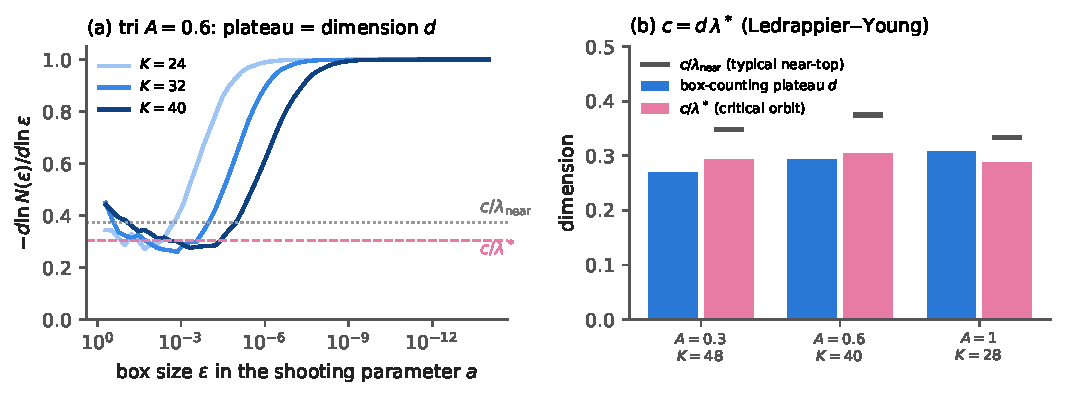
\includegraphics[width=\textwidth]{fig7_fractal.pdf}
\caption{The near-critical set $\{a:W_K(a)\ge\max W_K-A/2\}$ in the shooting parameter. (a) Local box-counting slope for the triangle model at $A=0.6$: a plateau at $d\approx0.28$--$0.29$ forms and widens with $K$, ending where the intervals are resolved (slope 1). Dashed: $c/\lambda^*$; dotted: $c/\lambda_{\rm near}$. (b) Plateau dimension against $c/\lambda^*$ (critical orbit) and $c/\lambda_{\rm near}$ (typical near-top state).}
\label{fig:fractal}
\end{figure}

\paragraph{Analogy.}
A finite complexity at threshold, with a marginal leading state ($\det H=0$), is the depinning analogue of the \emph{threshold} level of mean-field glasses (e.g.\ $p$-spin), where the complexity is positive and the dominant states are marginal.
The annealed picture, with the complexity vanishing continuously at $f_c^{\rm ann}$ ("topology trivialisation"), is instead the analogue of the ground state, where it vanishes.

\begin{table}[H]
\centering\footnotesize\setlength{\tabcolsep}{3.5pt}
\begin{tabular}{lcccccccc}
\toprule
model & $f_c^{\rm ann}$ & $f_{\rm sa}$ & $f_c$ (fits) & $d\varphi_q/d\tau|_{\tau\to\infty}$ & $c$ & $c/\Lambda(1)$ & $c_{\min}$ & $c_{\min}/\Lambda_{\rm st}$ \\
\midrule
\csname @@input\endcsname table_theory.tex
\bottomrule
\end{tabular}
\caption{Theory checks. $f_{\rm sa}$ is the amplitude-quenched bound, Eq.~\eqref{eq:bounds}. The large-$\tau$ slope of the quenched pressure is fitted on $18\le\tau A\le24$ (Gaussian: $\tau\sigma$). $c$ and $c_{\min}$ are the slopes in $K$ (four largest sizes) of $\langle\ln N\rangle$ and $\langle\ln N_{\min}\rangle$ at depth $A/2$ below the sample maximum.}
\label{tab:theory}
\end{table}

\begin{figure}[H]
\centering
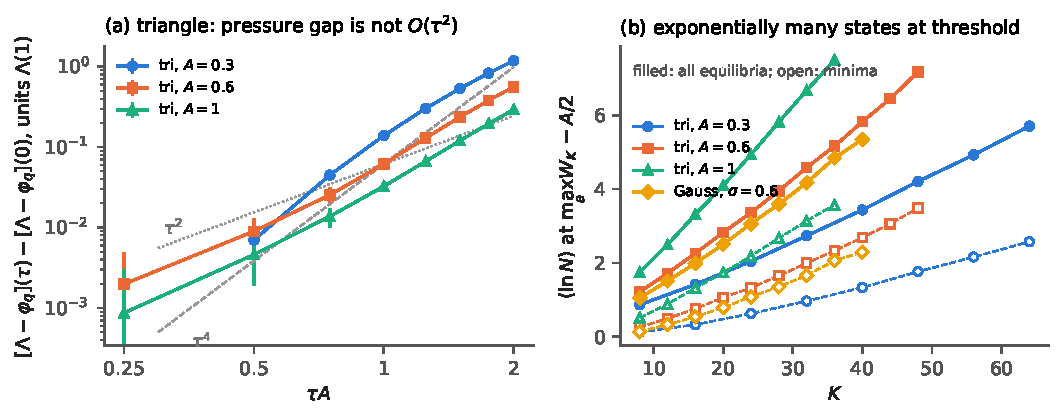
\includegraphics[width=\textwidth]{fig5_theory.pdf}
\caption{(a) Triangle models: the gap between annealed and quenched pressure, relative to $\tau=0$, against the $\tau^2$ and $\tau^4$ guides. (b) $\langle\ln N\rangle$ (filled) and $\langle\ln N_{\min}\rangle$ (open) at depth $A/2$ below the sample maximum, i.e.\ at a force $A/(2K)$ below the sample threshold. Linear growth in $K$ means exponentially many states at threshold.}
\label{fig:theory}
\end{figure}

\subsection{Strong pinning: a solvable limit}\label{sec:strong}

The dimension $d$, and hence $c$, has no closed form at weak pinning. The opposite limit is solvable.
Let the pinning stiffness $k=|V''|$ be large ($L_c=k^{-2/3}\ll1$). Near threshold the mean force must be close to $A$, so every site sits near a peak of its force.

Write $u_i=q_i+\sigma_is_i$, where
\begin{itemize}
\item $q_i=p_i+n_iP$ is a peak ($p_i=\phi_i+P/2$ for the triangle wave, $n_i\in\mathbb Z$),
\item $\sigma_i=\pm1$ is the side of the peak,
\item $s_i\ge0$ is the distance from it.
\end{itemize}
On either side the force is $A-ks_i$, so force balance $(\Delta_N^2u)_i=V_i'(u_i)-f$ reads
\begin{equation}
k\,s_i+\big(\Delta_N^2(\sigma s)\big)_i=b_i\equiv A-f-(\Delta_N^2q)_i .
\end{equation}
For $k\to\infty$, $s_i=b_i/k+O(k^{-2})$ independently of the signs, and this is admissible whenever every $b_i\ge0$.
Four consequences follow.

\begin{enumerate}
\item \textbf{Threshold.}
\begin{equation}
f_c=A-M^*,\qquad M^*=\min_{n\in\mathbb Z^K}\max_i(\Delta_N^2q)_i .
\end{equation}
Write the slopes as $w_j=q_{j+1}-q_j\in d_j+P\mathbb Z$, with $d_j=p_{j+1}-p_j$. The free ends require $w_0\le M$, $w_j-w_{j-1}\le M$ and $-w_{K-2}\le M$. Choosing the largest admissible slope at each step is optimal, so feasibility of a given $M$ is a single greedy pass (\texttt{minimax.py}).
The greedy increments are uniform on $(M-P,M]$, with drift $M-P/2$. A long chain is therefore feasible iff $M\ge P/2$, and
\begin{equation}
f_c\to A-\frac P2,\qquad \langle M^*\rangle-\frac P2\simeq-\frac2K,\qquad {\rm sd}\,f_c(K)=\frac{P}{\sqrt{12K}} .
\end{equation}
The minimax solver confirms all three up to $K=4096$ (Fig.~\ref{fig:strong}b). This explains the $K^{-1/2}$ sample-threshold fluctuations found throughout: they are those of a random walk with uniform increments of width $P$.
\item \textbf{The jump.} Just below $f_c$, all $2^K$ choices $\sigma\in\{\pm1\}^K$ are equilibria: each site sits left or right of its peak at the same force cost. Hence
\[
c\to\ln2 .
\]
\item \textbf{Minima.} The left side of a peak is stable ($V''=+k$) and the right side unstable. The Morse index is the number of right-side sites, only the all-left choice is a minimum, and
\[
c_{\min}\to0 .
\]
\item \textbf{Dimension.} The stretching per site is $\simeq\ln k$, so $d=c/\lambda^*\simeq\ln2/\ln k\to0$.
\end{enumerate}

\paragraph{An exact threshold formula for $k>2$.}
The leading-order argument can be made exact.
A site on the falling side of its peak has $V''=-k$, so the Hessian's diagonal entry there is $2-k$ ($1-k$ at a free end), and the configuration is unstable whenever $k>2$.
Hence, for $k>2$, \emph{the minima are exactly the configurations with every site on a rising branch}.
There $V_i'(u)=A+k(u-q_i)$ is linear, so each lift $n$ gives one equilibrium, $u-q=y-(A-f)/k$ with $y=(k-\Delta_N^2)^{-1}\Delta_N^2q_n$.
It is valid iff $\max y-\min y\le P/2$ and $A-f\ge k\max y$.
Since the depinning threshold is the largest force with a stable equilibrium,
\begin{equation}
f_c=A-\min_{n\in\mathbb Z^K}\;k\max_i\big[(k-\Delta_N^2)^{-1}\Delta_N^2q_n\big]_i\qquad(k>2),
\label{eq:fcexact}
\end{equation}
a minimax over integer lifts of a \emph{smoothed} curvature, which reduces to $M^*$ as $k\to\infty$.
Checked against exact bisection on $540$ samples ($k=3$ and $6$, $K=6$--$10$; \texttt{strong\_exact.py}), Eq.~\eqref{eq:fcexact} agrees to $3\times10^{-9}$, the bisection tolerance.

The curvature lattices decouple, $c_j\in e_j+P\mathbb Z$, the only global constraint is $\sum_jc_j=0$, and the kernel decays like $\rho^{|i-j|}$ with $\cosh\ln\rho^{-1}=1+k/2$.
So feasibility at a given $f$ is a dynamic programme over (running slope, last $2r$ curvatures), linear in $K$ (\texttt{fc\_dp}; banded kernel $r=2$, error $\sim10^{-2}$).
This gives the infinite-chain threshold where enumeration cannot reach (\texttt{strong\_scan.py}, $K$ up to $320$):

\begin{table}[H]
\centering\footnotesize
\begin{tabular}{lccccc}
\toprule
$k$ & 3 & 6 & 12 & 24 & 48 \\
\midrule
$f_c(\infty)-(A-P/2)$ & 0.780 & 0.489 & 0.279 & 0.151 & 0.075 \\
$\gamma=k[f_c-(A-P/2)]/P$ & 0.59 & 0.73 & 0.84 & 0.90 & 0.90 \\
$f_c^{\rm ann}-(A-P/2)$ & 1.270 & 1.264 & 1.264 & 1.264 & 1.264 \\
$f_c^{\rm ann}/f_c$ & 1.275 & 1.173 & 1.096 & 1.050 & 1.026 \\
${\rm sd}\,f_c(K)\sqrt K$ ($K=320$) & 0.63 & 0.77 & 0.89 & 0.97 & 1.00 \\
\bottomrule
\end{tabular}
\caption{Strong-pinning threshold from the exact minimax, Eq.~\eqref{eq:fcexact} ($P=4$, $A=k$). $f_c(\infty)$ is extrapolated as $f_c+a/K$ over $K\ge40$; at $K=16$ and $10$ the minimax reproduces the enumeration means ($1.87$ vs $1.86$ at $k=3$, $4.65$ vs $4.65$ at $k=6$).}
\label{tab:strong}
\end{table}

This yields concrete strong-pinning predictions:
\begin{equation}
f_c=A-\frac P2+\gamma\frac Pk+O(k^{-2}),\quad\gamma\to0.90\pm0.03;\qquad
f_c^{\rm ann}=A-\frac P2+0.316\,P;\qquad
{\rm sd}\,f_c\to\frac{P}{\sqrt{12K}} .
\end{equation}
A first-order expansion of the kernel gives $\gamma\approx1$: a site may take the next lattice value up when its neighbours have slack, which happens with probability $\simeq1/(k-2)$ and gains $P$ each time. The exact minimax gives $0.90$.
The annealed bound overshoots the true threshold by a \emph{constant} $0.316P$, set by $\Lambda(1)\simeq\ln k$ against the Cramér cost near the force edge. Only the ratio $f_c^{\rm ann}/f_c\to1$, because $A$ grows.

\paragraph{Test.}
Exact enumeration at $k=2$, $3$ and $6$ (\texttt{queue\_strong.sh}, $K\le20$, $16$ and $10$) bridges the two regimes (Fig.~\ref{fig:strong}a):
\begin{itemize}
\item \textbf{The jump rises toward $\ln2$:} $c=0.094$, $0.166$, $0.213$, $0.316$, $0.375$ and $0.501$ for $k=0.3$, $0.6$, $1$, $2$, $3$ and $6$, i.e.\ $72\%$ of $\ln2$ at $k=6$.
\item \textbf{Minima drop out:} $c_{\min}/c$ falls from $\approx0.55$ ($k\le1$) to $0.46$, $0.40$ and $0.19$.
\item \textbf{Weak-pinning side:} $c$ follows the continuum scaling $c\simeq0.22/L_c$, the same form as $\Sigma(0)=0.456/L_c$, so $c\simeq0.48\,\Sigma(0)$.
\item \textbf{Threshold:} the measured $\langle f_c\rangle$ approaches the leading order $A-M^*(K)$ from above, with a gap of $0.93$, $0.73$ and $0.45$ at $k=2$, $3$ and $6$, from the $O(P/k)$ freedom of sites to move off their peaks.
\end{itemize}

So the jump interpolates between a universal $0.22/L_c$ at weak pinning and exactly $\ln2$ at strong pinning.
At strong pinning its origin is explicit: the side of each peak is a free binary choice, and only the all-left choice is a minimum.
Weak pinning is the same mechanism with the binary choices diluted. Only a fraction of sites sit close enough to a peak, and that fraction sets $d$.

\begin{figure}[H]
\centering
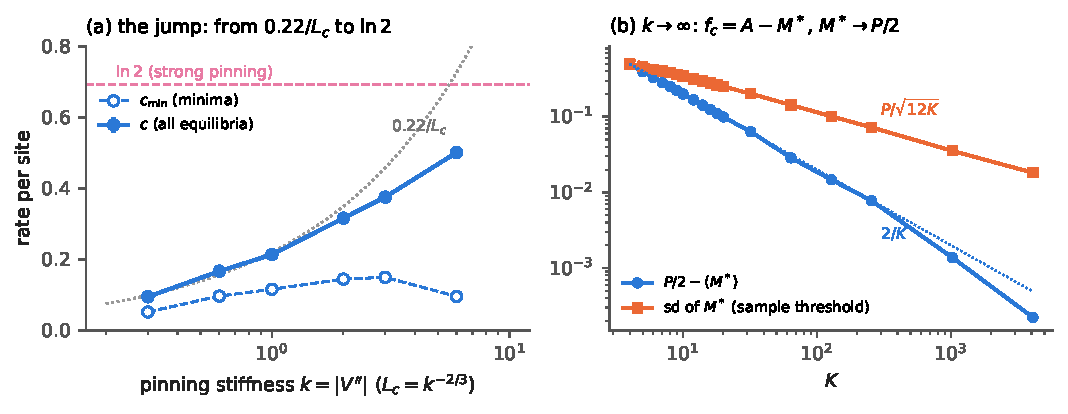
\includegraphics[width=\textwidth]{fig8_strong.pdf}
\caption{From weak to strong pinning. (a) The jump $c$ (filled) and $c_{\min}$ (open) against the pinning stiffness $k$, with the continuum scaling $0.22/L_c=0.22\,k^{2/3}$ (dotted) and the strong-pinning limit $\ln2$ (dashed). (b) Strong-pinning threshold $f_c=A-M^*$: the minimax $M^*$ tends to $P/2$ with a $2/K$ correction (dotted), and its sample-to-sample spread is $P/\sqrt{12K}$ (dashed).}
\label{fig:strong}
\end{figure}

\subsection{Transfer operators on the torus}\label{sec:torus}

The population picture of Sec.~7.3 is also a computational method that needs no enumeration.
On the torus $(u\bmod P,\,w\bmod P)$, the tilted curve-length measure evolves linearly, $\rho_{i+1}=\mathcal L_{\phi_i}\rho_i$, with one transport operator per site phase $\phi_i$, and $Z_K=\|\mathcal L_{\phi_{K-1}}\cdots\mathcal L_{\phi_0}\rho_0\|$. Hence
\begin{equation}
\varphi_q(\tau)=\lim_K K^{-1}\big\langle\ln\|\mathcal L_{\phi_{K-1}}\cdots\mathcal L_{\phi_0}\|\big\rangle,\qquad
\Lambda(\tau)=\ln\rho\big(\langle\mathcal L_\phi\rangle\big),
\label{eq:torus}
\end{equation}
the top Lyapunov exponent of a product of independent random positive operators, against the log spectral radius of their mean.
Since the curve's strands align with the unstable direction, one tangent direction per point suffices, carried as a line field.

We discretise $\rho$ on an $n\times n$ grid (bilinear transport, \texttt{torus.py}) and average $\ln m_i$ over one long run of $3000$ sites.
The grid smooths structure below $h=P/n$, which acts as weak noise. Merging strands closer than $h$ is harmless, because they share their future.
\begin{itemize}
\item \textbf{Bulk and onset.} The torus reproduces the enumeration's quenched pressure to three decimals up to $\tau A\approx1.5$, i.e.\ through the whole quenched--annealed separation (Fig.~\ref{fig:torus}a). It does so at $K\to\infty$ directly, with no finite-size extrapolation, at a cost independent of $K$.
\item \textbf{Frozen phase.} At large $\tau$ the edge is set by strand bundles thinner than $h$, and the grid overestimates it. As $h\to0$ the slope and intercept of the frozen asymptote converge toward the enumeration values $f_c=0.171$--$0.175$ and $c=0.166$ (Fig.~\ref{fig:torus}c). This independently confirms, at $K=\infty$, both the threshold and a positive jump $c$.
\end{itemize}

\paragraph{Exact decomposition of the gap.}
Conditioning on the past and averaging over the fresh phase,
\begin{equation}
\Lambda(\tau)-\varphi_q(\tau)=\underbrace{\big\langle\Lambda-\ln\langle m_i\rangle_\phi\big\rangle}_{\rm memory}
+\underbrace{\big\langle\ln\langle m_i\rangle_\phi-\langle\ln m_i\rangle_\phi\big\rangle}_{\rm one\text{-}step\ Jensen},
\end{equation}
which the torus evaluates exactly, step by step, with a phase quadrature.
The one-step Jensen term carries almost all of the gap. For example, at $A=0.6$ and $\tau A=3$ it is $0.479$ of $0.461$, while the memory term is $0.021$; the memory and Jensen parts need not add exactly to the directly measured gap, which is the noisier estimate.
Its second-order form $\tfrac12\langle{\rm Var}_\phi m_i/\langle m_i\rangle_\phi^2\rangle$, i.e.\ Eq.~\eqref{eq:jgap}, matches it within $1$--$2\%$ up to $\tau A=1.5$ and within $20\%$ at $\tau A=3$ (Fig.~\ref{fig:torus}b; resolution-stable to $5\%$ for $n=128$--$512$).
So the quenched--annealed gap is, quantitatively, the phase variance of the one-step growth factor. That variance is set by the non-uniformity of the tilted population in $u$, which grows continuously with $\tau$ (its participation ratio rises from $1.01$ at $\tau=0$ to $1.16$ at $\tau A=1$ and $8$ at $\tau A=12$).

\begin{figure}[H]
\centering
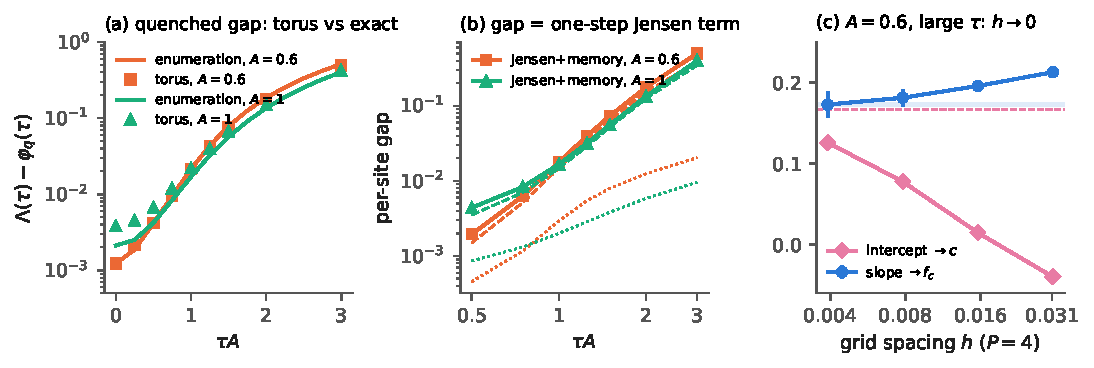
\includegraphics[width=\textwidth]{fig6_torus.pdf}
\caption{Transfer operators on the torus, Eq.~\eqref{eq:torus}. (a) $\Lambda-\varphi_q$ from the torus ($n=256$, markers) and from exact enumeration (lines). (b) Memory plus one-step Jensen term (markers), its second-order estimate $\tfrac12\langle{\rm Var}_\phi m\rangle$ (dashed) and the memory term alone (dotted). (c) Frozen asymptote at $A=0.6$ (from $\tau A=6$ and $12$) against grid spacing: slope (band: enumeration $f_c$) and intercept (dashed: enumeration $c$).}
\label{fig:torus}
\end{figure}

\subsection{Exact thresholds of long chains: no passing}\label{sec:relax}

Enumeration stops at $K\lesssim64$, and the threshold extrapolations of Table~\ref{tab:thr} differ by up to $4\%$ depending on the assumed form.
Here the threshold is computed exactly for chains of $K=1024$ sites, at every pinning strength.
The model is convex in the elastic coupling, so the no-passing rule (Middleton) holds: forward-only relaxation from $u\equiv0$ either stops in a stable configuration, or advances every site by a full period $P$. By the shift symmetry $u\to u+P$, the line then moves forever.
So ``pinned at $f$'' is decided exactly, and the sample threshold follows by bisection (\texttt{relax.py}).
Each local move solves $F_i=0$ exactly on the piecewise-linear force, so there is no time step and no tolerance beyond the bisection one ($10^{-7}A$).
This is the polynomial-time feasibility oracle of the exact formula $f_c=A-\min\max_iL_i$ of Sec.~\ref{sec:strong}, valid at all $k$.

\paragraph{Checks.}
\begin{itemize}
\item Against exact enumeration plus bisection on the same samples ($A=0.6$, $1$, $3$, short chains), the thresholds agree to $10^{-8}$.
\item At $k=3$ and $6$, the relaxation gives $f_c(\infty)=1.779$ and $4.492$. The independent minimax dynamic programme of Sec.~\ref{sec:strong} gives $1.780$ and $4.489$.
\item The means agree with the enumeration means of independent samples at every common size ($K=16$--$64$, $k=0.3$--$3$), within $1.5$ standard errors.
\end{itemize}

\begin{table}[H]
\centering\footnotesize
\begin{tabular}{lcccccc}
\toprule
$k=A$ & 0.3 & 0.6 & 1 & 2 & 3 & 6 \\
\midrule
$\langle f_c(1024)\rangle$ & 0.0686 & 0.1758 & 0.3474 & 0.9721 & 1.7823 & 4.4951 \\
$f_c(\infty)$ & 0.0682(8) & 0.1749(13) & 0.3460(20) & 0.970(3) & 1.779(4) & 4.492(5) \\
$f_c^{\rm ann}$ & 0.1084 & 0.2704 & 0.5240 & 1.3335 & 2.2696 & 5.2642 \\
$f_c^{\rm ann}/f_c$ & 1.59(2) & 1.55(1) & 1.51(1) & 1.375(5) & 1.275(3) & 1.172(1) \\
$f_c\,L_c^2=f_c\,k^{-4/3}$ & 0.339 & 0.346 & 0.346 & 0.385 & 0.411 & 0.412 \\
$f_c^{\rm ann}L_c^2$ & 0.540 & 0.534 & 0.524 & 0.529 & 0.525 & 0.483 \\
${\rm sd}\,f_c(K)\sqrt K$ ($K=1024$) & 0.10 & 0.20 & 0.31 & 0.54 & 0.61 & 0.84 \\
\bottomrule
\end{tabular}
\caption{Exact long-chain thresholds by no-passing relaxation ($P=4$; $600$ samples per $K\le256$, $300$ for $K=512$, $1024$). $f_c(\infty)$ is the fit $f_c+aK^{-3/4}$ over $K\ge64$; the error spans the fits with $K^{-1/2}$ and $K^{-1}$ plus the statistical error.}
\label{tab:relax}
\end{table}

\paragraph{Results.}
\begin{itemize}
\item \textbf{The ratio, exactly.} $f_c^{\rm ann}/f_c=1.59\pm0.02$ at $k=0.3$ ($L_c=2.2$), then $1.55$ and $1.51$ at $k=0.6$ and $1$. The extrapolation from $K=1024$ moves $f_c$ by only $0.5$--$1\%$, so this is no longer a matter of fit form. The $\nu=4/3$ extrapolation of the enumeration was too low; the front and free-$\nu$ fits were right.
\item \textbf{Continuum limit.} The weak-pinning thresholds follow Larkin scaling, $f_cL_c^2\simeq0.34$ and $f_c^{\rm ann}L_c^2\simeq0.53$, with lattice corrections of opposite sign (Table~\ref{tab:relax}). Extrapolating the ratio to $k\to0$, linearly or quadratically in $1/L_c$ or $1/L_c^2$, gives $1.60$--$1.70$. FLRT's dynamical $1.64\pm0.02$ is inside this range: our static, exact thresholds are consistent with it, and the remaining difference at finite $L_c$ is a lattice effect.
\item \textbf{One curve from weak to strong pinning.} The ratio falls monotonically with $k$ and joins the strong-pinning minimax at $k=3$--$6$, then follows $f_c^{\rm ann}/(A-P/2+0.90P/k)\to1$ (Fig.~\ref{fig:relax}b). The annealed overshoot $f_c^{\rm ann}-f_c$ grows from $0.04$ at $k=0.3$ to $0.77$ at $k=6$, and saturates at $0.316P$.
\item \textbf{Fluctuations.} ${\rm sd}\,f_c(K)\sqrt K$ is constant from $K=16$ to $1024$ at every $k$: the $K^{-1/2}$ law of Sec.~\ref{sec:theory} holds over two decades, and tends to $P/\sqrt{12}$ only slowly at strong pinning.
\end{itemize}

\begin{figure}[H]
\centering
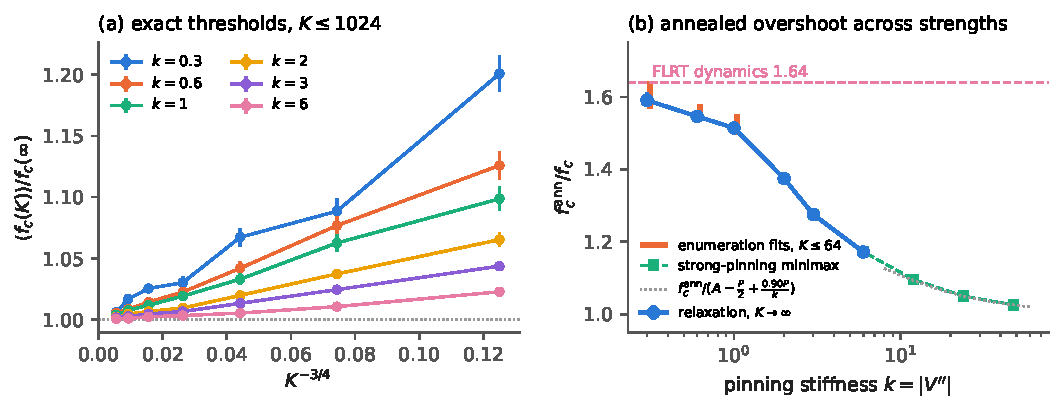
\includegraphics[width=\textwidth]{fig9_relax.pdf}
\caption{Exact thresholds by no-passing relaxation. (a) $\langle f_c(K)\rangle/f_c(\infty)$ against $K^{-3/4}$ for $K=16$--$1024$. (b) $f_c^{\rm ann}/f_c$ against the pinning stiffness: relaxation (circles; bars span the extrapolation forms), enumeration fits of Table~\ref{tab:thr} (bars at $k\le1$), the strong-pinning minimax (squares) and its asymptote (dotted). Dashed: FLRT's dynamical $1.64$.}
\label{fig:relax}
\end{figure}

\section{Open questions}

\begin{itemize}
\item \textbf{The non-uniformity spectrum.} The gap is the phase variance of the one-step growth, Eq.~\eqref{eq:jgap}. A closed computation of the stationary $\langle|\hat\rho_n|^2\rangle$, for example a linear-response treatment of the tilt plus shear mixing, would give $\Sq(f)$ analytically. Second moments alone will not do, because stable-close strands lock even at $\tau=0$, where the quenched and annealed pressures coincide.
\item \textbf{Expansion in $1/k$.} The strong-pinning limit is exact at leading order. The first corrections, sites moving by $O(P/k)$ off their peaks with signs no longer decoupled, should give $c=\ln2-O(1/k)$ and the shift of $f_c$, and connect to the weak-pinning dimension.
\item \textbf{The dimension $d$.} With $c=d\lambda^*$, the open quantity is the unstable dimension $d\approx0.28$ of the critical measure. For a hyperbolic set it solves a Bowen equation, $P_{\max}(-d\ln J^u)=0$, with the pressure restricted to the force-maximising orbits. Whether $d$ is universal in the continuum limit, and the analogous $d_{\min}=c_{\min}/\lambda^*\approx0.16$ for minima, are open.
\item \textbf{Continuum limit.} The torus method costs the same at weak disorder, so it can give the universal curve $\Sq(f)L_c$ against $f/f_c^{\rm ann}$ and the onset as $L_c\to\infty$. A finer grid, or adaptive refinement near the edge, is needed for $f_c$ and $c$.
\item \textbf{Weaker disorder.} The relaxation needs no enumeration and takes seconds per sample at $K=1024$, so $k=0.1$--$0.2$ ($L_c=3$--$5$) is in reach. It would pin down the continuum ratio, now $1.60$--$1.70$, and test Larkin scaling of $f_c$ directly. The same code with Gaussian amplitudes would treat FLRT's own model.
\item \textbf{Longer blocks.} The block bound, Eq.~\eqref{eq:blockbound}, should become tight as $\ell\to\infty$, but its planted-strand estimator needs populations $\gg e^{\gamma\ell}$. A transfer operator on densities of entry states under the block-tilted law, or importance sampling of the entry state, would remove that tail and test how fast $B_\ell\to\varphi_q$.
\item \textbf{Sizes.} Larger $K$ near $f\approx0.75f_c$, and an overlap measure in the bulk of the chain rather than at the free end, would sharpen the onset.
\item \textbf{Medium size.} Here the period of the medium is fixed while $K$ grows, as in FLRT's torus. A medium of period $\gg K^\zeta$ would test whether the localisation factor survives in an unbounded medium.
\end{itemize}

\paragraph{Reproduce.}\sloppy
All steps run from this folder:
\begin{itemize}
\item \texttt{./queue\_levels.sh} and \texttt{./queue\_cos.sh} write the exact counts to \texttt{data\_levels/};
\item \texttt{python3 profile\_center.py --A 0.6 --K 8 12 16 20 24 28 32} computes the level-profile centre and width;
\item \texttt{./queue.sh} and \texttt{python3 verify\_tilt.py} give the direct runs and the tilt-symmetry checks;
\item \texttt{python3 semi\_annealed.py} computes the amplitude-quenched rate $\Lambda_q(\tau)$;
\item \texttt{python3 analyze.py} writes \texttt{statistics.json}, the tables and Figs.~1--4;
\item \texttt{python3 theory.py} writes \texttt{theory.json}, Table~\ref{tab:theory} and Figs.~\ref{fig:theory}, \ref{fig:torus};
\item \texttt{python3 torus\_runs.py} writes \texttt{torus.json} and \texttt{torus\_decomposition.json} (transfer operators on the torus);
\item \texttt{python3 lyap\_leader.py} writes \texttt{lyap\_leader.json} (stretching of the critical configuration);
\item \texttt{python3 strong\_exact.py} tests the exact threshold formula, and \texttt{python3 strong\_scan.py} gives the infinite-chain strong-pinning thresholds (\texttt{strong\_exact.json}, \texttt{strong\_scan.json});
\item \texttt{./queue\_strong.sh} and \texttt{python3 minimax.py} give the strong-pinning runs and the minimax threshold (\texttt{strong\_pinning.json} is written by the analysis in \texttt{theory.py});
\item \texttt{python3 replica.py} writes \texttt{replica.json} (pair moment $\Lambda_2(\tau)$ by population dynamics; \texttt{--check} tests $n=1$ against the exact $\Lambda$); \texttt{python3 theory.py --replica-only} writes \texttt{replica\_summary.json} and Fig.~\ref{fig:replica};
\item \texttt{python3 fracbound.py} and \texttt{python3 fracbound2.py} write \texttt{fracbound.json} and \texttt{fracbound2.json} (change-of-measure bounds, iid and Markov tilts; \texttt{fracbound.py --check} tests $h=1$ against the exact $\Lambda$);
\item \texttt{python3 blockbound.py} writes \texttt{blockbound.json} (block-tilt bounds with the exact polygon $Z_b$, two population sizes per point; \texttt{--check} tests $\lambda=0$ against the exact $\Lambda$); \texttt{python3 theory.py --block-only} writes \texttt{block\_summary.json} and Fig.~\ref{fig:block};
\item \texttt{python3 relax.py} writes \texttt{relax.json} (exact thresholds by no-passing relaxation, $K\le1024$); \texttt{python3 theory.py --relax-only} writes \texttt{relax\_summary.json} (the extrapolations of Table~\ref{tab:relax}) and Fig.~\ref{fig:relax};
\item \texttt{python3 fractal\_top.py} writes \texttt{fractal\_top.json} (box counting of the near-critical set; Fig.~\ref{fig:fractal} is drawn by \texttt{theory.py}).
\end{itemize}
The library code is in \texttt{qcount.py} (enumeration) and \texttt{annealed.py} (exact annealed quantities).

\end{document}
